\section{Soundness}\label{sec:tcsoundness}
In this section, we prove the soundness of the type system presented in Section \ref{section:typeruless}. That is, we prove a subject reduction result and that a typing of a process provides a bound on the parallel complexity of the process. We first augment the definition of annotated processes and extend the type rules.
%
\subsection{Augmented language and type system}
In the type system from Chapter \ref{ch:bgts}, subtyping rules for processes and expressions are used extensively to bound parallel compositions and to prove a subject reduction property. However, such use of subtyping is notoriously difficult to implement, as there may be an infinite number of subtypes. Consider for instance a parallel composition of two processes $P$ and $Q$ that are typed as $\varphi;\Phi;\Gamma\vdash P \triangleleft 10 - i$ and $\varphi;\Phi;\Gamma\vdash Q \triangleleft i^2 - 100i$, respectively. These complexities are both functions of $i$ and clearly intersect. It is not trivial to find a common subtype of these indices in practice, and for more complex indices, it quickly becomes intractable.\\

In the case of subject reduction, where we have a reduction $P \Longrightarrow Q$, Baillot and Ghyselen \cite{BaillotGhyselen2021} use a subtyping rule for expressions extensively. In particular, upon synchronization of an input and an output on some channel, we require that the expressions to be transmitted can be typed as super types of the message types of the channel. Thus, upon reduction we use the subtyping rule to assign the message types to the expressions. In this case, we use information from the typing of $P$ to \textit{guide} subtyping in the typing of $Q$, and so by augmenting the reduction relation with annotations, we can implement subtyping. An alternative is to permit the subtyping rule for expressions to prove the soundness of the type system, and then omit it from the implementation, i.e. we simply reject processes that cannot be typed without using the subtyping rule. This is a valid compromise, as it avoids needless cluttering of the reduction relation with annotations, and we are usually not interested in using the subject reduction property in practice. That is, we need only type a process prior to any reduction, presuming the type system is sound. Therefore, we take this approach, introducing the subtyping rule for expressions below.
\begin{align*}
    \runa{S-subsumption}\;\infrule{\varphi;\Phi;\Gamma\vdash e : S\quad \varphi;\Phi\vdash S \sqsubseteq T}{\varphi;\Phi;\Gamma\vdash e : T}
\end{align*}
As reduction may reduce ticks, subsequently modifying the typing of a process, we need a \textit{delaying} property to prove a subject reduction result. That is, it must be safe to increase the bound in a typing, so long as all bounds on synchronizations in the type context are correspondingly increased (We write this as $\uparrow^I\!\!\Gamma$ when we increase bounds by $I$, as defined in Definition \ref{def:delayy}). Such a property is proved by induction on the type rules.
%
\begin{defi}[Delaying]\label{def:delayy}
We define the delaying $\uparrow^I\!\!T$ of a type $T$ by an index $I$ by the rules 
\begin{align*}
    \uparrow^L\!\!\texttt{Nat}[I,J] =&\; \texttt{Nat}[I,J]\\
    \uparrow^L\!\!\texttt{ch}^\sigma_I(\widetilde{T}) =&\; \texttt{ch}^\sigma_{I+L}(\widetilde{T})\\
    \uparrow^L\!\!\forall_I\widetilde{i}.\texttt{serv}^\sigma_K(\widetilde{T}) =&\; \forall_{I+L}\widetilde{i}.\texttt{serv}^\sigma_K(\widetilde{T})
\end{align*}
We extend delaying to contexts such that for all $v\in\texttt{dom}(\Gamma)$ such that $\Gamma(v)=T$ we have that $(\uparrow^I\!\!\Gamma)(v)=\uparrow^I\!\!T$.
\end{defi}
%
However, this turns out to be problematic due to type annotations on restrictions. That is, in the clause for restriction, we can assume that $\varphi;\Phi;\Gamma\vdash (\nu a :T) P \triangleleft \kappa$ from which we also have $\varphi;\Phi;\Gamma,a:T\vdash P \triangleleft \kappa$, and by induction we obtain $\varphi;\Phi;\uparrow^I\!\!\Gamma,a:\uparrow^I\!\!T\vdash P \triangleleft \kappa + I$, which unfortunately does not comply with the type annotation in $(\nu a:T) P$. Without a delaying property, we are (to our knowledge) unable to preserve a typing upon reduction, i.e. either the needed type context or assignable combined complexity (possibly both) changes. Unfortunately, this is an insufficient condition to prove that a bound on an assigned combined complexity $\kappa$ is in fact a bound on the span, as constant changes to expressions $I$ or $J$ in a judgement $\varphi;\Phi;\Gamma\vdash I \bowtie J$ is enough to sometimes (even for linear functions) fail a judgement. An example of this is depicted in Figure \ref{fig:srnecess}, showcasing that a strong subject reduction property is crucial to prove soundness.\\ %Consider for instance the two univariate linear functions below\\

\begin{figure}
    \centering
    \begin{minipage}{.5\textwidth}
    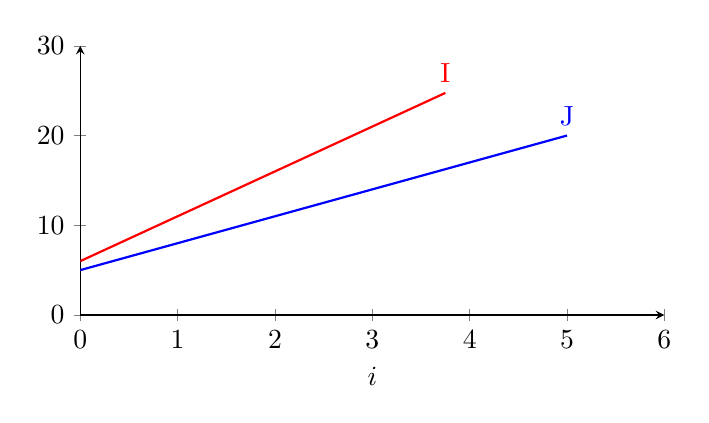
\begin{tikzpicture}
        \begin{axis}[
            axis lines = left,
            xlabel = \(i\),
            ylabel = {},
            domain = 0:5,
            xmin=0,
            xmax=6,
            ymin=0,
            ymax=30,
            restrict y to domain=0:25,
            height=5cm,
            width=9cm,
        ]
        \addplot[thick, color=red]{5*x+6} node[above,pos=1] {I};
        \addplot[thick, color=blue]{3*x+5} node[above,pos=1] {J};
    \end{axis}
    \end{tikzpicture}
\end{minipage}%
\begin{minipage}{.5\textwidth}
    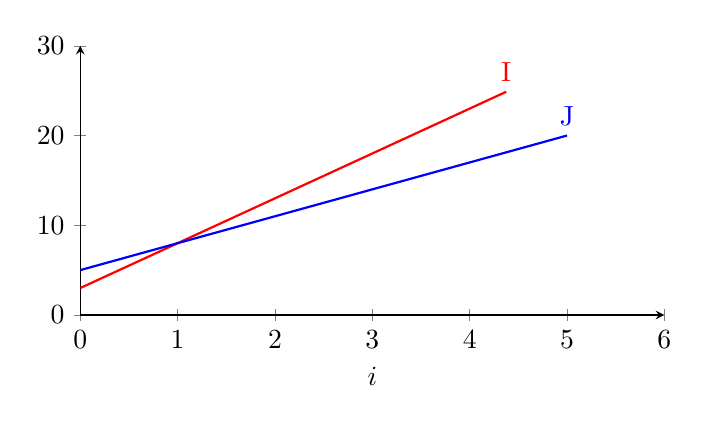
\begin{tikzpicture}
        \begin{axis}[
            axis lines = left,
            xlabel = \(i\),
            ylabel = {},
            domain = 0:5,
            xmin=0,
            xmax=6,
            ymin=0,
            ymax=30,
            restrict y to domain=0:25,
            height=5cm,
            width=9cm,
        ]
        \addplot[thick, color=red]{5*x+3} node[above,pos=1] {I};
        \addplot[thick, color=blue]{3*x+5} node[above,pos=1] {J};
    \end{axis}
    \end{tikzpicture}
\end{minipage}
%[width=5cm]%
    \caption{The image on the left depicts two linear indices $I = 5i+6$ and $J= 3i+5$ as functions of $i$ that do not intersect in the non-negative valuation space of $i$. On the right, we subtract $3$ from $I$, shifting the intersection of $I$ and $J$ into the non-negative valuation space. Thus, $\{i\};\cdot\vDash J \leq I$ but $\{i\};\cdot\nvDash J \leq I-3$. }
    \label{fig:srnecess}
\end{figure}
%
%\includegraphics[width=13cm]{image.png}\\
%Subtracting $3$ from $f$ is enough to shift the intersection of $f$ and $g$ into the non-negative valuation space. Thus, to prove the soundness of an implementation of the type system, it is crucial to have a strong subject reduction property.\\

As we are not interested in actually using a subject reduction property in practice, we can introduce two versions of the implementation: One with type annotations on restrictions, and one without. That is, one without a subject reduction property, and one with a subject reduction property. Intuitively, if $\varphi;\Phi;\Gamma\vdash P \triangleleft \kappa$ by the type system with annotations, then also $\varphi;\Phi;\Gamma\vdash P \triangleleft \kappa$ by the type system without annotations, and so it suffices to prove soundness for the type system without type annotations, to show that any bound on $\kappa$ is an upper bound on the span. Thus, in the remainder of this section, we assume that restrictions do not have type annotations.

%As our restrictions have type annotations, and as annotations advance the time of a context, the structural congruence definition must be augmented to prove a subject congruence result. Consider for instance the process $n : \newvar{a : \texttt{ch}^\sigma_I(\widetilde{T})}{\inputch{a}{\widetilde{v}}{}{P}}$ with some typing $\varphi;\Phi;\Gamma\vdash n : \newvar{a : \texttt{ch}^\sigma_I(\widetilde{T})}{\inputch{a}{\widetilde{v}}{}{P}} \triangleleft \kappa + I + n$ with $\varphi;\Phi;\downarrow_n\!\!\Gamma,a:\texttt{ch}^\sigma_I(\widetilde{T})\vdash \inputch{a}{\widetilde{v}}{}{P} \triangleleft \kappa + I$. Then $\newvar{a : \texttt{ch}^\sigma_I(\widetilde{T})}{n : \inputch{a}{\widetilde{v}}{}{P}}$ is not typable whenever $\varphi;\Phi\nvDash n\leq I$. However, we can quickly verify that $\varphi;\Phi;\Gamma\vdash \newvar{a : \texttt{ch}^\sigma_{I+n}(\widetilde{T})}{n : \inputch{a}{\widetilde{v}}{}{P}} \triangleleft \kappa + I + n$. Thus, if we \textit{delay} or advance the time of a type annotation upon a time annotation in and out (respectively) of the scope of the corresponding restriction, then the subject congruence property holds. Therefore, we formalize \textit{delaying} of types in Definition \ref{def:delayy}. 
%
%if intuitively $\varphi;\Phi;\Gamma,a:\text{delay}(\varphi,\Phi,\Gamma,\iota)\vdash \iota : P \triangleleft K$ where $I$ is the advancement of time imposed by $\iota$.
%

%
% We augment the structural congruence rule $\runa{SC-ares}$ correspondingly
% \begin{align*}
%     \runa{SC-ares}\; n : \newvar{a:T}{P} \equiv \newvar{a:T^{+n}}{n : P}
% \end{align*}
% %
% Moreover, we assume the subsequent rules for restrictions are extended with type annotations. Note that the changes to $\runa{SC-ares}$ do not affect the existence of a canonical form, as we can always apply $\runa{SC-ares}$ from left to right (As we do in the proof of Lemma \ref{lemma:anncannform}), as $T^{+n}$ is defined for any $n$ whenever $T$ is defined.
% %
% % \begin{align*}
%     \text{delay}(\varphi,\Phi,\Gamma,\epsilon, T) =&\; T \\
%     %
%     \text{delay}(\varphi,\Phi,\Gamma,(1,\widetilde{\iota}), T) =&\; \text{delay}(\varphi,\Phi,\susume{\Gamma}{\varphi}{\Phi}{1},\widetilde{\iota},T+1)\\
%     %
%     \text{delay}(\varphi,\Phi,(\Gamma,a:\texttt{ch}^\sigma_I(\widetilde{T})),(a(\widetilde{v})^n_\epsilon,\widetilde{\iota}), T) =&\; \text{delay}(\varphi,\Phi,(\susume{\Gamma}{\varphi}{\Phi}{I},a:\texttt{ch}^\sigma_0(\widetilde{T})),\widetilde{\iota},T+I)\\
%     %
%     \text{delay}(\varphi,\Phi,(\Gamma,a:\forall_I\widetilde{i}.\texttt{serv}^\sigma_K(\widetilde{T})),(a(\widetilde{v})^n_{\widetilde{e}},\widetilde{\iota}), T) =&\; \text{delay}(\varphi,\Phi,(\susume{\Gamma}{\varphi}{\Phi}{I},a:\forall_I\widetilde{i}.\texttt{serv}^\sigma_K(\widetilde{T})),\widetilde{\iota},T+I)
% \end{align*}
%\end{defi}
%

% We now define the local complexity of an augmented process based on its prefix of annotations in Definition \ref{def:lcbg}. Specifically, a tick has a cost of one in time complexity, and so the $1$-annotation adds one to the local complexity. Channel annotations $a(\widetilde{v})^n_{\widetilde{e}}$ are more complex, as we treat the constant $n$ similarly to the time $I$ of a channel type $\texttt{ch}^\sigma_I(\widetilde{T})$, in that it is relative. For instance, in a typing $\varphi;\Phi;\cdot,a:\texttt{ch}^{\{\texttt{in}\}}_I(\widetilde{T}),b:\texttt{ch}^{\{\texttt{out}\}}_J(\widetilde{S}) \vdash \inputch{a}{\widetilde{v}}{}{\tick\asyncoutputch{b}{\widetilde{e}}{}} \triangleleft J$, we type $\asyncoutputch{b}{\widetilde{e}}{}$ under the context $\cdot,a:\texttt{ch}^{\{\texttt{in}\}}_0(\widetilde{T}),b:\texttt{ch}^{\{\texttt{out}\}}_{J-I-1}(\widetilde{S})$, and so the bound on the complexity is $I+1+(J-I-1)=J$ as $\varphi;\Phi\vDash I+1 \leq J$ by definition of advancement of time. In the same sense, each constant added to the local complexity is subtracted from all succeeding channel annotations, and so local complexity has the following properties. If $\mathcal{C}_\ell(\widetilde{\iota} : G) \geq n$ then $\mathcal{C}_\ell(\widetilde{\iota} : a(\widetilde{v})^n_{\widetilde{e}} : G)=\mathcal{C}_\ell(\widetilde{\iota} : G)$ and if $\mathcal{C}_\ell(\widetilde{\iota} : G) \leq n$ then $\mathcal{C}_\ell(\widetilde{\iota} : a(\widetilde{v})^n_{\widetilde{e}} : G)=n$. Thus, if we are careful with how channel annotations are introduced, then this definition of local complexity is equivalent to the one in Definition \ref{def:bglcsim}.
% %
% \begin{defi}[Local complexity]\label{def:lcbg}
% We define the local complexity $\mathcal{C}_\ell(P)$ of an augmented process $P$ inductively
% %\begin{align*}
% \begin{alignat*}{3}
%     \mathcal{C}_\ell(1 : P) =&&\; 1 + \mathcal{C}_\ell(P^{-1})\qquad\qquad\qquad\kern1em (1 : P)^{-n} =&&\; 1 : P^{-n}\kern3em\;\;\\
%     \mathcal{C}_\ell(a(\widetilde{v})^n_{\widetilde{e}} : P) =&&\; n + \mathcal{C}_\ell(P^{-n})\qquad\qquad\kern0.5em (a(\widetilde{v})^m_{\widetilde{e}} : P)^{-n} =&&\; a(\widetilde{v})^{m-n}_{\widetilde{e}} : P^{-n}\;\\
%     \mathcal{C}_\ell(P \mid Q) =&&\; \text{max}(\mathcal{C}_\ell(P),\mathcal{C}_\ell(Q))\qquad\qquad (P\mid Q)^{-n} =&&\; P^{-n} \mid Q^{-n}\kern2em\\
%     \mathcal{C}_\ell(\newvar{a : T}{P}) =&&\; \mathcal{C}_\ell(P)\qquad\qquad\qquad\kern1em (\newvar{a:T}{_{\widetilde{\iota}}\; P})^{-n} =&&\; \newvar{a:T}{_{\widetilde{\iota}}\; P^{-n}}\;\;\;\\
%     \mathcal{C}_\ell(G) =&&\; 0 \qquad\qquad\qquad\kern8em G^{-n} =&&\; G\kern6em
% \end{alignat*}
% \end{defi}
% As expressions may now be annotated with variables, we must be careful when transmitting an expression over a channel. That is, the annotated variable may be bound in a channel annotation, and so it may be free in the process that receives the expression. To account for this, we introduce the notation $\circledcirc e$ in Definition \ref{def:annotrembg} that represents the expression $e$ with all annotations removed. As annotations solely guide subtyping, we can deduce that if we can assign some type $T$ to $e$, then we can assign a super type of $T$ to $\circledcirc e$. We formalize this result in Section \ref{sec:intermelemmabg}.
% \begin{defi}\label{def:annotrembg}
% We define the notation $\circledcirc e$ to denote $e$ without annotations, defined inductively by the rules
% \begin{align*}
%     \circledcirc e_\theta = \circledcirc e\kern2em  \circledcirc\! 0 = 0\kern2em\circledcirc \succc{e} = \s(\circledcirc e)\kern2em \circledcirc\! v = v
%     %\circledcirc 0 =&\; 0\\
%     %\circledcirc v =&\; v
% \end{align*}
% \end{defi}
% %
% In Definition \ref{tab:parallelredurules}, we now introduce the parallel reduction relation $\Longrightarrow$ for augmented processes. Tick prefixes reduce to $1$-annotations by rule $\runa{PR-tick}$. For pattern matches on a natural of the form $\succc{e}_{\widetilde{\theta}}$, we substitute $e_{\succc{e}_{\widetilde{\theta}}}$ for the variable bound in the successor pattern. Here, the annotation provides information about the typing of $\succc{e}$ prior to reduction, such that we can type $e$ accordingly subject to subtyping. The most notable rules are $\runa{PR-rep}$ and $\runa{PR-comm}$ that synchronize annotated inputs and outputs on servers and normal channels, respectively. We annotate the continuation of the input with the annotation prefix of the input extended with a channel annotation marked with the maximum of the local complexities of the prefixes of the input and output. Thus, the local complexity of the new annotation prefix is equal to the local complexity of the parallel composition prior to reduction. We substitute $(\circledcirc \widetilde{e})_{\widetilde{v}}$ for the variables bound in the input $\widetilde{v}$, where $\widetilde{e}$ are the expressions of the output and $(\circledcirc \widetilde{e})_{\widetilde{v}}=(\circledcirc e_1)_{v_1},\dots,(\circledcirc e_n)_{v_n}$. Here, we use the notation $\circledcirc e$ to remove annotations that potentially contain variables bound in the annotation prefix of the output, i.e. they are free in the input process. We annotate the expressions with the variables they replace, to provide information for subtyping when typing the process after reduction.\\

% %
% \begin{table*}[ht]
%     \centering
%     \begin{framed}\vspace{-1em}\begin{align*}
%         &\kern0em\runa{PR-rep}\;\;\condinfrule{}{\parcomp{\widetilde{\iota}_1 : \;\bang{\inputch{a}{\widetilde{v}}{}{P}}}{\widetilde{\iota}_2 : \asyncoutputch{a}{\widetilde{e}}{}} \Longrightarrow \parcomp{\widetilde{\iota}_1 : \;\bang{\inputch{a}{\widetilde{v}}{}{P}}}{\widetilde{\iota}_2 : a(\widetilde{v})^n_{\widetilde{e}} :\subst{P}{\widetilde{v}\mapsto (\circledcirc\widetilde{e})_{\widetilde{v}}}}}{\!\!\!\!\!\!\!\!\!\!\text{where}\; n = \text{max}(\mathcal{C}_\ell(\widetilde{\iota}_1 : \nil),\mathcal{C}_\ell(\widetilde{\iota}_2 : \nil))}\\
%         %
%         &\kern0em\runa{PR-comm}\;\;\condinfrule{}{\widetilde{\iota}_1 :\inputch{a}{\widetilde{v}}{}{P}
%         \mid 
%         \widetilde{\iota}_2 : \asyncoutputch{a}{\widetilde{e}}{} \Longrightarrow \widetilde{\iota}_1 : a(\widetilde{v})^n_{\epsilon} : \subst{P}{\widetilde{v}\mapsto (\circledcirc\widetilde{e})_{\widetilde{v}}}}{\text{where}\; n = \text{max}(\mathcal{C}_\ell(\widetilde{\iota}_1 : \nil),\mathcal{C}_\ell(\widetilde{\iota}_2 : \nil))}\\[-1em]
%         %
%         &\kern0em\runa{PR-zero}\;\;\infrule{}{\match{0_{\widetilde{\theta}}}{P}{x}{Q} \Longrightarrow P}
%         %
%         \kern6em\runa{PR-par}\;\;\infrule{P \Longrightarrow Q}{\parcomp{P}{R} \Longrightarrow \parcomp{Q}{R}}
%         \\[-1em]
%         %
%         &\kern0em\runa{PR-succ}\;\;\infrule{}{\match{\succc{e}_{\widetilde{\theta}}}{P}{x}{Q} \Longrightarrow Q[x \mapsto e_{\succc{e}_{\widetilde{\theta}}}]}  \\[-1em]
%         %
%         %\kern0em\runa{PR-empty}\;\;\infrule{}{\texttt{match}\; []_{\widetilde{\theta}}\; \{ [] \mapsto P; x :: y \mapsto Q \} \Longrightarrow P} \\[-1em]
%         %
%         &\runa{PR-annot}\infrule{P \Longrightarrow Q}{\iota : P \Longrightarrow \iota : Q}\kern6em \runa{PR-res}\;\;\infrule{P \Longrightarrow Q}{\newvar{a : T}{_{\widetilde{\iota}}\; P} \Longrightarrow \newvar{a : T}{_{\widetilde{\iota}}\;Q}}
%         \\[-1em]
%         %
%         %\kern7em\runa{PR-cons}\;\;\infrule{}{\texttt{match}\; (e :: e')_{\widetilde{\theta}}\; \{ [] \mapsto P; x :: y \mapsto Q \} \Longrightarrow Q[x \mapsto e,y \mapsto e_{\widetilde{\theta},-1}']}\\[-1em]
%         %
%         %\kern3em\runa{R-par}\;\;\infrule{P \longrightarrow Q}{\parcomp{P}{R} \longrightarrow \parcomp{Q}{R}} \kern-0em \runa{R-res}\;\;\infrule{P \longrightarrow Q}{\newvar{a}{P} \longrightarrow \newvar{a}{Q}}\\
%         %
%         &\kern4em\runa{PR-struct}\;\;\infrule{P \equiv P'\quad P' \Longrightarrow Q'\quad Q' \equiv Q}{P \Longrightarrow Q} \kern1em \runa{PR-tick}\;\;\infrule{}{\tick P \Longrightarrow 1 : P}\kern5.5em\text{ }
%     \end{align*}\end{framed}
%     \smallskip
%     \caption{The parallel reduction rules defining $\Longrightarrow$.}
%     \label{tab:parallelredurules}
% \end{table*}
% %
% %
% Finally, in Definition \ref{def:pcbga} we define the parallel complexity of an augmented process $P$ to be equal to the maximum local complexity amongst process $P$ and processes that $P$ can reduce to.
% %
% \begin{defi}[Parallel complexity]\label{def:pcbga}
% Let $P$ be an augmented process, then we define the parallel complexity of $P$ as
% \begin{align*}
%     \mathcal{C}_\mathcal{P}(P) = \text{max}\{ \mathcal{C}_\ell(Q) \mid P \Longrightarrow^* Q \}
% \end{align*}
% where $\Longrightarrow^*$ is the transitive and reflexive closure of $\Longrightarrow$.
% \end{defi}

% \subsection{Annotated type rules}\label{sec:anntyperulebg}

% % $\varphi;\Phi;\Gamma;\Delta\vdash^m_J P \triangleleft K$ $\varphi;\Phi;\Gamma;\Delta\vdash e : T$.

% \begin{table*}[ht]
%     \begin{framed}\vspace{-1em}\begin{align*}
%         &\kern-6em
%         \runa{S-zero}\;\infrule{}{\varphi;\Phi;\Gamma;\Delta\vdash\withtype{0}{\typenat[0,0]}}\kern0em
%         \runa{S-succ}\;\infrule{\varphi;\Phi;\Gamma;\Delta \vdash \withtype{e}{\typenat[I, J]}}{\varphi;\Phi;\Gamma;\Delta \vdash \withtype{\succc{e}}{\typenat[I + 1, J + 1]}}\\[-1em]
%         %
%         %&\kern-8em\runa{S-empty}\;\infrule{}{\varphi;\Phi;\Gamma\vdash_\Delta\withtype{[]}{\texttt{List}[0,0](\mathcal{B})}}\kern0em
%         %\runa{S-cons}\;\infrule{\varphi;\Phi;\Gamma\vdash_{\Delta} e : \mathcal{B} \quad\varphi;\Phi;\Gamma \vdash_\Delta \withtype{e'}{\texttt{List}[I, J](\mathcal{B}')}}{\varphi;\Phi;\Gamma \vdash_\Delta \withtype{e :: e'}{\texttt{List}[I + 1, J + 1](\mathcal{B} \uplus_{\varphi;\Phi} \mathcal{B}')}}\\[-1em]
%         %
%         &%\runa{S-cons-2}\;\infrule{\varphi;\Phi;\Gamma\vdash e : \mathcal{B} \quad\varphi;\Phi;\Gamma \vdash \withtype{e'}{\texttt{List}[0, 0](\mathcal{B}')}}{\varphi;\Phi;\Gamma \vdash \withtype{e :: e'}{\texttt{List}[1, 1](\mathcal{B})}}\quad\quad\quad\quad\quad\quad\quad
%         %
%         \kern-6em\runa{S-var}\;\infrule{}{\varphi;\Phi;\Gamma, \withtype{v}{T};\Delta \vdash \withtype{v}{T}}
%         \runa{S-avar}\;\infrule{\varphi;\Phi;\Gamma;\Delta,v:T\vdash e : S\quad \varphi;\Phi\vdash S \sqsubseteq T}{\varphi;\Phi;\Gamma;\Delta,v:T\vdash e_v : T}\\
%         %
%         &\kern-9em\runa{S-strength}\; \infrule{\varphi;\Phi;\Gamma;\Delta\vdash e : \texttt{Nat}[I',J']\quad \varphi;\Phi;\Gamma;\Delta\vdash e' : \texttt{Nat}[I,J]\quad \varphi;\Phi\vdash \texttt{Nat}[I',J']\sqsubseteq \texttt{Nat}[I-1,J-1]}{\varphi;\Phi;\Gamma;\Delta\vdash e_{e'} : \texttt{Nat}[I-1,J-1]}%\\
%         %
%         %&\kern-10em\runa{S-strength-2}\; \infrule{\varphi;\Phi;\Gamma\vdash_\emptyset \circledcirc e : \texttt{List}[I',J'](\mathcal{B}')\quad \varphi;\Phi;\Gamma\vdash_\Delta e : \texttt{List}[I,J](\mathcal{B})\quad \varphi;\Phi\vdash \texttt{List}[I',J'](\mathcal{B}')\sqsubseteq \texttt{List}[I-1,J-1](\mathcal{B})}{\varphi;\Phi;\Gamma\vdash_\Delta e_{-1} : \texttt{List}[I-1,J-1](\mathcal{B})}
%     \end{align*}\vspace{-1em}\end{framed}
%     \smallskip
%     \caption{Extended type rules for expressions.}
%     \label{tab:sizedannottypedexpressiontypes}
% \end{table*}

% \begin{table*}[!ht]
%     \begin{framed}\vspace{-1em}\begin{align*}
%         &\kern15em\\[-2em] % Stretch frame
%         &\kern0em\runa{SA-nil}\infrule{}{\varphi;\Phi;\Gamma;\Delta \vdash_{J} \withcomplex{\nil}{\{0\}}}
%         %
%         \kern3em\runa{SA-tick}\;\infrule{\varphi;\Phi;\susumesim{\Gamma}{1};\downarrow_1\!\!\Delta\vdash_{J+1} P \triangleleft \kappa}{\varphi;\Phi;\Gamma;\Delta\vdash_{J} \tick P \triangleleft \kappa + 1}\\[-1em]
%         %
%         &\kern-0em\runa{SA-match}\;\infrule{
%         \begin{matrix}
%             \varphi;\Phi;\Gamma;\Delta \vdash \withtype{e}{\natinterval{I}{J}}\quad \varphi;\Phi, I \leq 0;\Gamma;\Delta \vdash_{L} \withcomplex{P}{\kappa} \\
%             \varphi;\Phi, J \geq 1;\Gamma, \withtype{x}{\natinterval{I-1}{J-1}};\Delta \vdash_{L} \withcomplex{Q}{\kappa'}
%         \end{matrix}}{\varphi;\Phi;\Gamma;\Delta \vdash_{L} \withcomplex{\match{e}{P}{x}{Q}}{\text{basis}(\varphi,\Phi,\kappa\cup\kappa')}}\\[-1em]
%         %
%         %&\kern-0em\runa{S-nmatch-2}\;\infrule{
%         %\begin{matrix}
%         %    \varphi;\Phi;\Gamma \vdash \withtype{e}{\natinterval{I}{J}} \quad \varphi;\Phi\vDash K \leq K' \\
%         %    \varphi;\Phi, I \leq 0;\Gamma \vdash \withcomplex{P}{K} \quad \varphi;\Phi, J \geq 1;\Gamma, \withtype{x}{\natinterval{I-1}{J-1}} \vdash \withcomplex{Q}{K'}
%         %\end{matrix}}{\varphi;\Phi;\Gamma \vdash \withcomplex{\match{e}{P}{x}{Q}}{K'}}\\[-1em]
%         %
%         %&\kern-0em\runa{SA-lmatch}\;\condinfrule{
%         %\begin{matrix}
%         %    \varphi;\Phi;\Gamma \vdash \withtype{e}{\texttt{List}[I,J](\mathcal{B})} \quad \varphi;\Phi, I \leq 0;\Gamma \vdash^m_L \withcomplex{P}{K} \\
%         %    \varphi;\Phi, J \geq 1;\Gamma, \withtype{x}{\mathcal{B}},y : \texttt{List}[I-1,J-1](\mathcal{B}) \vdash^m_L \withcomplex{Q}{K'}
%         %\end{matrix}}{\varphi;\Phi;\Gamma \vdash^m_L \withcomplex{\texttt{match}\;e\;\{ [] \mapsto P;\; x :: y \mapsto Q \}}{L}}{\text{where}\quad L = \left\{
% %\begin{matrix}
% %    K & \text{if}\; \varphi;\Phi\vDash K' \leq K   \\
% %    K' & \text{if}\; \varphi;\Phi\vDash K \leq K'  %\\
%     %K+K' & \text{otherwise}
% %\end{matrix}
% %\right.}\\[-1em]
%         %
%         %&\kern-0em\runa{S-lmatch-2}\;\infrule{
%         %\begin{matrix}
%         %    \varphi;\Phi;\Gamma \vdash \withtype{e}{\texttt{List}[I,J](\mathcal{B})} \quad \varphi;\Phi\vDash K \leq K' \\
%         %    \varphi;\Phi, I \leq 0;\Gamma \vdash \withcomplex{P}{K} \quad \varphi;\Phi, J \geq 1;\Gamma, \withtype{x}{\mathcal{B}},y : \texttt{List}[I-1,J-1](\mathcal{B}) \vdash \withcomplex{Q}{K'}
%       % \end{matrix}}{\varphi;\Phi;\Gamma \vdash \withcomplex{\texttt{match}\;e\;\{ [] \mapsto P;\; x :: y \mapsto Q \}}{K'}}\\[-1em]
%         %
%         %&\kern4em\runa{SA-par}\;\condinfrule{\varphi;\Phi;\Gamma;\Delta\vdash^m_{J} P \triangleleft K\quad \varphi;\Phi;\Gamma;\Delta\vdash^m_{J} Q \triangleleft K'}{\varphi;\Phi;\Gamma;\Delta\vdash^m_{J} \parcomp{P}{Q} \triangleleft L}{\text{where}\quad L = \left\{
% %\begin{matrix}
% %    K & \text{if}\; \varphi;\Phi\vDash K' \leq K   \\
% %    K' & \text{if}\; \varphi;\Phi\vDash K \leq K'  %\\
%     %K+K' & \text{otherwise}
% %\end{matrix}
% %\right.}\\[-1em]
% %
% &\kern-0em\runa{SA-par}\;\infrule{\varphi;\Phi;\Gamma;\Delta\vdash_J P \triangleleft \kappa\quad \varphi;\Phi;\Gamma;\Delta\vdash_J Q \triangleleft \kappa'}{\varphi;\Phi;\Gamma;\Delta\vdash_J P \mid Q \triangleleft \text{basis}(\varphi,\Phi,\kappa\cup\kappa')}
% %
% \kern8em\runa{SA-nu}\;\infrule{\varphi;\Phi;\Gamma,\withtype{a}{\text{delay}(\varphi,\Phi,\Gamma,\widetilde{\iota},T)};\Delta \vdash_{J} \withcomplex{P}{\kappa}}{\varphi;\Phi;\Gamma;\Delta \vdash_{J} \newvar{a: T}{_{\widetilde{\iota}}\; P}\triangleleft \kappa} \\[-1em]
% %
% %&\runa{SA-par-fail}\;\condinfrule{\varphi;\Phi;\Gamma;\Delta\vdash^m_J P \triangleleft K;\kappa\quad \varphi;\Phi;\Gamma;\Delta\vdash^m_J Q \triangleleft K';\kappa'\quad \forall L\in\kappa''.\exists L'\in\kappa''.\varphi;\Phi\nvDash L' \leq L}{\varphi;\Phi;\Gamma;\Delta\vdash^m_J P \mid Q \triangleleft 0; \kappa''}{\kappa'' = \kappa \cup \kappa' \cup \{K,K'\}}    \\[-1em]
% %
%         %
%         %&\kern4em\runa{S-par-2}\;\infrule{\varphi;\Phi;\Gamma\vdash P \triangleleft K\quad \varphi;\Phi;\Gamma\vdash Q \triangleleft K'\quad \varphi;\Phi\vDash K \leq K'}{\varphi;\Phi;\Gamma\vdash \parcomp{P}{Q} \triangleleft K'}\\[-1em]
%         %
%         &\kern-0em\runa{SA-iserv}\;\infrule{\texttt{in}\in\sigma\quad \varphi,\widetilde{i};\Phi;\text{ready}(\varphi,\Phi,\susumesim{\Gamma}{I}),a:\forall_0\widetilde{i}.\texttt{serv}^{\sigma\cap\{\texttt{out}\}}_K(\widetilde{T}),\widetilde{v} : \widetilde{T};\text{ready}(\varphi,\Phi,\susumesim{\Delta}{I})\vdash_{J+I} P \triangleleft \kappa\quad\varphi,\widetilde{i};\Phi\vDash \kappa \leq K}{\varphi;\Phi;\Gamma,a:\forall_I\widetilde{i}.\texttt{serv}^\sigma_K(\widetilde{T});\Delta\vdash_{J}\; \bang\inputch{a}{\widetilde{v}}{}{P}\triangleleft \{I\}}\\[-1em]
%         %
%         &\kern-0em\runa{SA-ich}\;\infrule{\texttt{in}\in\sigma\quad \varphi;\Phi;\susumesim{\Gamma}{I},a:\texttt{ch}_0^\sigma(\widetilde{T}),\widetilde{v} : \widetilde{T};\Delta\vdash_{J+I} P \triangleleft \kappa}{\varphi;\Phi;\Gamma,a:\texttt{ch}_I^\sigma(\widetilde{T});\Delta\vdash_{J} \inputch{a}{\widetilde{v}}{}{P}\triangleleft \kappa + I}\\[-1em]
%         %
%         &\kern-0em\runa{SA-och}\;\infrule{\texttt{out}\in \sigma\quad \varphi;\Phi;\susumesim{\Gamma}{I};\Delta\vdash \widetilde{e} : \widetilde{T}\quad \varphi;\Phi\vdash\widetilde{T}\sqsubseteq\widetilde{S}}{\varphi;\Phi;\Gamma,a:\texttt{ch}^{\sigma}_I(\widetilde{S});\Delta\vdash_{J} \asyncoutputch{a}{\widetilde{e}}{} \triangleleft \{I\}}
%         %
%         \kern12em\runa{SA-atick}\;\infrule{\varphi;\Phi;\downarrow_1\!\!\Gamma;\downarrow_1\!\!\Delta\vdash_{J+1} P \triangleleft \kappa}{\varphi;\Phi;\Gamma;\Delta\vdash_{J} 1 : P \triangleleft \kappa + 1}
%         \\[-1em]
%         %
%         &\kern0em\runa{SA-oserv}\;\infrule{\texttt{out} \in \sigma\quad \varphi;\Phi;\susumesim{\Gamma}{I};\cdot\vdash \circledcirc\widetilde{e} : \widetilde{T}\quad \text{instantiate}(\widetilde{i},\widetilde{T})=\{\widetilde{J}/\widetilde{i}\}\quad  \varphi;\Phi\vdash\widetilde{T}\sqsubseteq\widetilde{S}\{\widetilde{J}/\widetilde{i}\}}{\varphi;\Phi;\Gamma,a:\forall_I\widetilde{i}.\texttt{serv}_K^\sigma(\widetilde{S});\Delta\vdash_{L} \asyncoutputch{a}{\widetilde{e}}{} \triangleleft \{K\!\substi{\widetilde{J}}{\widetilde{i}} + I\}}\\[-1em]
%         %
%         &\kern0em\runa{SA-aich}\;\infrule{\varphi;\Phi\vDash n \leq I + J\quad \varphi;\Phi;\downarrow_I\!\!\Gamma,a:\texttt{ch}^\sigma_0(\widetilde{T});\downarrow_I\!\!\Delta,\widetilde{v}:\widetilde{T}\vdash_{J+I} P \triangleleft \kappa}{\varphi;\Phi;\Gamma,a : \texttt{ch}^\sigma_I(\widetilde{T});\Delta\vdash_{J} a(\widetilde{v})^n_\epsilon : P \triangleleft \kappa + I}\\
%         %
%         &\kern0em\runa{SA-aiserv}\;\infrule{
%         \begin{matrix}
%             \varphi;\Phi\vDash n \leq I + J\quad \varphi;\Phi;\downarrow_I\!\!\Gamma;\cdot\vdash \circledcirc\widetilde{e} : \widetilde{S} \quad \text{instantiate}(\widetilde{i},\widetilde{S})=\{\widetilde{L}/\widetilde{i}\}\\ 
%             %\varphi;\Phi\vdash \widetilde{S} \sqsubseteq \widetilde{T}\{\widetilde{L}/\widetilde{i}\}\quad
%             %
%             \varphi;\Phi;\downarrow_I\!\!\Gamma,a:\forall_0\widetilde{i}.\texttt{serv}^{\sigma\cap\{\texttt{out}\}}_K(\widetilde{T});\downarrow_I\!\!\Delta,\widetilde{v}:\widetilde{T}\{\widetilde{L}/\widetilde{i}\}\vdash_{J+I} P \triangleleft \kappa %\quad\varphi,\widetilde{i};\Phi\vDash \kappa \leq K\{\widetilde{L}/\widetilde{i}\}
%         \end{matrix}
%         }{\varphi;\Phi;\Gamma, a : \forall_I\widetilde{i}.\texttt{serv}^\sigma_K(\widetilde{T});\Delta\vdash_{J} a(\widetilde{v})^n_{\widetilde{e}} : P \triangleleft \kappa + I}
%     \end{align*}\vspace{-1em}\end{framed}
%     \smallskip
%     \caption{Sized typing rules for parallel complexity of annotated processes.}
%     \label{tab:sizedannotatedprocesstypingrules}
% \end{table*}

\subsection{Intermediary lemmas}\label{sec:intermelemmabg}
We are now ready to present the soundness results. We first prove some intermediary lemmas that we use for the main results. We first prove some useful properties with respect to delaying in Lemma \ref{lemma:delayingg}. We use the first point in the clause of $\runa{SC-ares}$ in the proof of subject congruence. We use the second and third points for the proof of subject reduction, namely for synchronizations on channels, where we preserve the maximal local complexity amongst an input and output, and so we may need to \textit{delay} the type context.
%
\begin{lemma}[Delaying]\label{lemma:delayingg}\text{ }
\begin{enumerate}
    \item $\susume{\uparrow^I\!\!T}{\varphi}{\Phi}{I}=T$.
    \item If $\varphi;\Phi;\Gamma\vdash e : T$ then $\varphi;\Phi;\uparrow^I\!\!\Gamma\vdash e : \uparrow^I\!\!T$.
    \item If $\varphi;\Phi;\Gamma\vdash P \triangleleft \kappa$ then $\varphi;\Phi;\uparrow^I\!\!\Gamma\vdash P \triangleleft \kappa + I$.
\end{enumerate}
\begin{proof} Point $1$ is straightforward. Point $2$ and $3$ are proved by induction on the type rules of expressions and processes, respectively.
\end{proof}
\end{lemma}
%
We next prove that advancement of time is additive. This result is integral to subject congruence, namely for $\runa{SC-sum}$ that allows us to sum two annotations, and correspondingly split one annotation into two. 
%
\begin{lemma}[Additive advancement of time]\label{lemma:addsusume}
Let $\Phi$ be a set of constraints with unknowns in $\varphi$ and let $T$ be a type then $\susume{\susume{T}{\varphi}{\Phi}{J}}{\varphi}{\Phi}{I} =\; \susume{T}{\varphi}{\Phi}{I+J}$.
 \begin{proof} On the structure of $T$. The proof is shown in Appendix \ref{app:sizedtypesoundness}.
%     \begin{description}
%     \item[$(\susume{\susume{\mathcal{B}}{\varphi}{\Phi}{J}}{\varphi}{\Phi}{I})$] obtained directly from  $\susume{\mathcal{B}}{\varphi}{\Phi}{J} = \mathcal{B}$ and $\susume{\mathcal{B}}{\varphi}{\Phi}{I} = \mathcal{B}$.
%     %
%     \item[$(\susume{\susume{\texttt{ch}^\sigma_L(\widetilde{T})}{\varphi}{\Phi}{J}}{\varphi}{\Phi}{I})$] We either have that
%     \begin{enumerate}
%         \item $\varphi;\Phi\vDash J \leq L$ and so we have that $\susume{\texttt{ch}^\sigma_L(\widetilde{T})}{\varphi}{\Phi}{J}=\texttt{ch}^\sigma_{L-J}(\widetilde{T})$. Then if $\varphi;\Phi\vDash I \leq L-J$ we also have $\varphi;\Phi\vDash I+J \leq L$ as $\varphi;\Phi\vDash J \leq L$, and so we obtain $\susume{\susume{\texttt{ch}^\sigma_L(\widetilde{T})}{\varphi}{\Phi}{J}}{\varphi}{\Phi}{I}=\susume{\texttt{ch}^\sigma_L(\widetilde{T})}{\varphi}{\Phi}{I+J}=\texttt{ch}^\sigma_{L-(I+J)}(\widetilde{T})$. Otherwise, we have that $\varphi;\Phi\nvDash I \leq L-J$, implying that $\varphi;\Phi\nvDash I+J \leq L$ as $\varphi;\Phi\vDash J \leq L$, and so we obtain $\susume{\susume{\texttt{ch}^\sigma_L(\widetilde{T})}{\varphi}{\Phi}{J}}{\varphi}{\Phi}{I}=\susume{\texttt{ch}^\sigma_L(\widetilde{T})}{\varphi}{\Phi}{I+J}=\texttt{ch}^\emptyset_{L-(I+J)}(\widetilde{T})$.
%         %
%         \item $\varphi;\Phi\nvDash J \leq L$ and so we have that $\susume{\texttt{ch}^\sigma_L(\widetilde{T})}{\varphi}{\Phi}{J}=\texttt{ch}^\emptyset_{L-J}(\widetilde{T})$ and $\susume{\texttt{ch}^\emptyset_{L-J}(\widetilde{T})}{\varphi}{\Phi}{I}=\texttt{ch}^\emptyset_{(L-J)-I}(\widetilde{T})$. It follows from the fact that $I$ is non-negative that also $\varphi;\Phi\nvDash I+J \leq L$ and so we obtain $\susume{\susume{\texttt{ch}^\sigma_L(\widetilde{T})}{\varphi}{\Phi}{J}}{\varphi}{\Phi}{I}=\texttt{ch}^\emptyset_{L-(J+I)}(\widetilde{T})=\texttt{ch}^\emptyset_{(L-J)-I}(\widetilde{T})$.
%     \end{enumerate}
%     %
%     \item[$(\susume{\susume{\forall_L\widetilde{i}.\texttt{serv}^\sigma_K(\widetilde{T})}{\varphi}{\Phi}{J}}{\varphi}{\Phi}{I})$] We either have that
%     \begin{enumerate}
%         \item $\varphi;\Phi\vDash J \leq L$ and so we have that $\susume{\forall_L\widetilde{i}.\texttt{serv}^\sigma_K(\widetilde{T})}{\varphi}{\Phi}{J}=\forall_{L-J}\widetilde{i}.\texttt{serv}^\sigma_K(\widetilde{T})$. Then if $\varphi;\Phi\vDash I \leq L-J$ we also have $\varphi;\Phi\vDash I+J \leq L$ as $\varphi;\Phi\vDash J \leq L$, and so we obtain $\susume{\susume{\forall_L\widetilde{i}.\texttt{serv}^\sigma_K(\widetilde{T})}{\varphi}{\Phi}{J}}{\varphi}{\Phi}{I}=\susume{\forall_L\widetilde{i}.\texttt{serv}^\sigma_K(\widetilde{T})}{\varphi}{\Phi}{I+J}=\forall_{L-(I+J)}\widetilde{i}.\texttt{serv}^\sigma_K(\widetilde{T})$. Otherwise, we have that $\varphi;\Phi\nvDash I \leq L-J$, implying that $\varphi;\Phi\nvDash I+J \leq L$ as $\varphi;\Phi\vDash J \leq L$, and so we obtain $\susume{\susume{\forall_L\widetilde{i}.\texttt{serv}^\sigma_K(\widetilde{T})}{\varphi}{\Phi}{J}}{\varphi}{\Phi}{I}=\susume{\forall_L\widetilde{i}.\texttt{serv}^\sigma_K(\widetilde{T})}{\varphi}{\Phi}{I+J}=\forall_{L-(I+J)}\widetilde{i}.\texttt{serv}^{\sigma\cap\{\texttt{out}\}}_K(\widetilde{T})$.
%         %
%         \item $\varphi;\Phi\nvDash J \leq L$ and so we have that $\susume{\forall_L\widetilde{i}.\texttt{serv}^\sigma_K(\widetilde{T})}{\varphi}{\Phi}{J}=\forall_{L-J}\widetilde{i}.\texttt{serv}^{\sigma\cap\{\texttt{out}\}}_K(\widetilde{T})$ and $\susume{\forall_{L-J}\widetilde{i}.\texttt{serv}^{\sigma\cap\{\texttt{out}\}}_K(\widetilde{T})}{\varphi}{\Phi}{I}=\forall_{(L-J)-I}\widetilde{i}.\texttt{serv}^{\sigma\cap\{\texttt{out}\}}_K(\widetilde{T})$. It follows from the fact that $I$ is non-negative that also $\varphi;\Phi\nvDash I+J \leq L$ and so we obtain $\susume{\susume{\forall_L\widetilde{i}.\texttt{serv}^\sigma_K(\widetilde{T})}{\varphi}{\Phi}{J}}{\varphi}{\Phi}{I}=\\forall_{L-(I+J)}\widetilde{i}.\texttt{serv}^{\sigma\cap\{\texttt{out}\}}_K(\widetilde{T})=\forall_{(L-J)-I}\widetilde{i}.\texttt{serv}^{\sigma\cap\{\texttt{out}\}}_K(\widetilde{T})$.
%     \end{enumerate}
%     \end{description}
\end{proof}
\end{lemma}
%
We now prove the usual weakening and strengthening lemmas in Lemma \ref{lemma:weakening} and Lemma \ref{lemma:strengthening}, respectively. In this work, we can weaken and strengthen sets of constraints and type contexts. That is, we can safely introduce new constraints or type associations, and discard constraints that are covered by the remaining constraints, as well as type associations for variables that are not free in a corresponding expression or process. As a consequence of type rule $\runa{S-subsumption}$, it is also safe to use subtyping on contexts.
%
\begin{lemma}[Weakening]\label{lemma:weakening}
Let $\Gamma$ and $\Gamma'$ be disjoint contexts. Then
\begin{enumerate}
    \item If $\varphi;\Phi;\Gamma\vdash e : T$ then $\varphi,\varphi';\Phi,\Phi';\Gamma,\Gamma'\vdash e : T$.
    %
    %\item If $\varphi;\Phi;\Gamma;\Delta\vdash^m_{J} P \triangleleft K$ and $n\leq m$ then also $\varphi;\Phi;\Gamma;\Delta\vdash^n_J P \triangleleft K$.
    %
    \item If $\varphi;\Phi;\Gamma\vdash P \triangleleft \kappa$ then $\varphi,\varphi';\Phi,\Phi';\Gamma,\Gamma'\vdash P \triangleleft \kappa$.
    %
    \item If $\varphi;\Phi;\Gamma\vdash e : T$ and $\varphi;\Phi\vdash \Delta \sqsubseteq \Gamma$ then $\varphi;\Phi;\Delta\vdash e : T$.
    %
    \item If $\varphi;\Phi;\Gamma\vdash P \triangleleft \kappa$ and $\varphi;\Phi\vdash \Delta \sqsubseteq \Gamma$ then $\varphi;\Phi;\Delta\vdash P \triangleleft \kappa$.
    %
    % \item If $\varphi;\Phi;\Gamma,a:\texttt{ch}^\sigma_I(\widetilde{T})\vdash P \triangleleft \kappa$ and $\sigma \subseteq \sigma'$ then also $\varphi;\Phi;\Gamma,a:\texttt{ch}^{\sigma'}_I(\widetilde{T})\vdash P \triangleleft \kappa$. 
    % %
    % \item If $\varphi;\Phi;\Gamma,a:\forall_I\widetilde{i}.\texttt{serv}_L^\sigma(\widetilde{T})\vdash P \triangleleft \kappa$ and $\sigma \subseteq \sigma'$ then also $\varphi;\Phi;\Gamma,a:\forall_I\widetilde{i}.\texttt{serv}_L^{\sigma'}(\widetilde{T})\vdash P \triangleleft \kappa$. 
\end{enumerate}
\begin{proof} Point $1$ and point $2$ are proved by induction on the type rules of expressions and processes, respectively. Point $3$ is proved by induction on the type rules of expressions, and point $4$ follows from point $3$.
\end{proof}
\end{lemma}

\begin{lemma}[Strengthening]\label{lemma:strengthening} Let $\Phi$ and $\Phi'$ be sets of constraints on $\varphi$ such that $\varphi;\Phi\vDash C$ for all $C\in\Phi'$. Then
\begin{enumerate}
    \item If $\varphi;(\Phi,\Phi')\vDash C'$ then also $\varphi;\Phi\vDash C'$.
    \item If $\varphi;(\Phi,\Phi')\vdash S \sqsubseteq T$ then also $\varphi;\Phi\vdash S \sqsubseteq T$.
    \item If $\susume{T}{\varphi}{(\Phi,\Phi')}{I}$ then also $\susume{T}{\varphi}{\Phi}{I}$.
    \item If $\varphi;\Phi,\Phi';\Gamma,\Gamma'\vdash e : T$ and the names in $\Gamma'$ are not free in $e$ then $\varphi;\Phi;\Gamma\vdash e : T$.
    \item If $\varphi;\Phi,\Phi';\Gamma,\Gamma'\vdash P \triangleleft \kappa$ and the names in $\Gamma'$ are not free in $P$ then $\varphi;\Phi;\Gamma\vdash P \triangleleft \kappa$.
\end{enumerate}
% If $\varphi;\Phi,\Phi';\Gamma,\Gamma';\Delta,\Delta'\vdash_J P \triangleleft \kappa$ such that $\varphi;\Phi\vDash C$ for all $C\in\Phi'$ and the names in $\Gamma'$ and $\Delta'$ are not free in $P$ then $\varphi;\Phi;\Gamma;\Delta\vdash_J P \triangleleft \kappa$.
\begin{proof} Point $1$ follows directly from $\varphi;\Phi\vDash C$ for all $C\in\Phi'$, i.e. $\Phi'$ imposes no further constraints on $\varphi$ given $\Phi$. Point $2$ is proved by induction on the subtyping rules. Point $4$ is proved by induction on the type rules of expressions using point $2$. Point $5$ is proved by induction on the type rules of processes using point $3$ and point $4$.
    %
 \end{proof}
 \end{lemma}
%
In the case of synchronization of a replicated input and an output on a server, we \textit{instantiate} the continuation of the input, by substituting expressions of the output for variables bound in the input. Similarly, the message types of the server are subject to index substitution, as per type rule $\runa{S-oserv}$. Thus, to prove a subject reduction property, we need to show that a well-typed process is also well-typed subject to index substitution. We prove this in Lemma \ref{lemma:isbg}. Notably, the inverse of point $2$ does not hold, as a judgement that does not hold prior to index substitution may be satisfied after. Consider for instance the judgement $\{i,j\};\cdot\nvDash i \leq j$ that clearly fails, as we do not constraint valuations of $i$ and $j$. However, the judgement $\{i\};\cdot\vDash i \leq j\{j/i\}$ is satisfied by the reflexive property of $\leq$. This explains the need for a weaker result with respect to point $6$. That is, we may use type rule $\runa{S-par}$ or $\runa{S-match}$ in the typing of a process $P$, such that the combined complexity is derived using the basis function, where complexity $K$ is discarded if a judgement of the form $\varphi;\Phi\vDash K \leq K'$ holds. Thus, after index substitution, we may be able to discard further complexity bounds.
%
\begin{lemma}[Index substitution]\label{lemma:isbg}
Let $\varphi$ be a set of index variables with $i\notin\varphi$, and let $J$ be an index with unknowns in $\varphi$. Then
\begin{enumerate}
    \item $[\![I\{J/i\}]\!]_\rho = [\![I]\!]_{\rho[i \mapsto [\![J]\!]_\rho]}$.
    \item If $(\varphi,i);\Phi\vDash C$ then $\varphi;\Phi\{J/i\}\vDash C\{J/i\}$.
    \item If $(\varphi,i);\Phi\vdash T \sqsubseteq S$ then $\varphi;\Phi\{J/i\}\vdash T\{J/i\} \sqsubseteq S\{J/i\}$.
    \item If $(\varphi,i);\Phi;\Gamma\vdash e : T$ then $\varphi;\Phi\{J/i\};\Gamma\{J/i\}\vdash e : T\{J/i\}$.
    %
    \item $\varphi;\Phi\{J/i\}\vdash\; \susume{T\{J/i\}}{\varphi}{\Phi\{J/i\}}{I\{J/i\}} \sqsubseteq\; \susume{T}{(\varphi,i)}{\Phi}{I}\{J/i\}$.
    %
    % \item $\susume{\texttt{ch}^\sigma_{I\{L/i\}}(\widetilde{T}\{L/i\})}{\varphi}{\Phi\{L/i\}}{J\{L/i\}}=\texttt{ch}^{\sigma'}_{(I-J)\{L/i\}}(\widetilde{T}\{L/i\})$ and $(\susume{\texttt{ch}^\sigma_I(\widetilde{T})}{\varphi,i}{\Phi}{J})\{L/i\} = \texttt{ch}^{\sigma''}_{(I-J)\{L/i\}}(\widetilde{T}\{L/i\})$ with $\sigma''\subseteq \sigma' \subseteq \sigma$.
    % %
    % \item $\susume{\forall_{I\{L/i\}}\widetilde{j}.\texttt{serv}^\sigma_{K\{L/i\}}(\widetilde{T}\{L/i\})}{\varphi}{\Phi\{L/i\}}{J\{L/i\}}=\forall_{(I-J)\{L/i\}}\widetilde{j}.\texttt{serv}^{\sigma'}_{K\{L/i\}}(\widetilde{T}\{L/i\})$ and $(\susume{\forall_I\widetilde{j}.\texttt{serv}^\sigma_K(\widetilde{T})}{\varphi,i}{\Phi}{J})\{L/i\} = \forall_{(I-J)\{L/i\}}\widetilde{j}.\texttt{serv}^{\sigma''}_{K\{L/i\}}(\widetilde{T}\{L/i\})$ with $\sigma''\subseteq \sigma' \subseteq \sigma$.
    %
    \item If $(\varphi,i);\Phi;\Gamma\vdash P \triangleleft \kappa$ then $\varphi;\Phi\{J/i\};\Gamma\{J/i\}\vdash P \triangleleft \kappa'\{J/i\}$ with $\varphi;\Phi\{J/i\}\vdash \kappa\{J/i\} = \kappa'\{J/i\}$.
\end{enumerate}
\begin{proof} Point $1$ is proved by induction on $I$ using the definition of interpretations of indices. Point $2$ is a direct consequence of point $1$. Point $3$ and $4$ are proved by induction on the subtyping rules and type rules for expressions, respectively, using point $2$. We use point $3$ to prove point $4$. Point $5$ is useful for point $6$ and follows from point $2$. Point $6$ is proved by induction on the type rules of processes, utilizing point $3$, $4$ and $5$.
\end{proof}
\end{lemma}
%
%
% \begin{lemma}\label{lemma:annotrembg}
% If $\varphi;\Phi;\Gamma;\Delta\vdash e : T$ then $\varphi;\Phi;\Gamma;\cdot\vdash \circledcirc e : S$ with $\varphi;\Phi\vdash S \sqsubseteq T$.
% \begin{proof} By induction on $e$. The proof is shown in Appendix \ref{app:sizedtypesoundness}.% We only show the interesting cases
%     % \begin{description}
%     % %
%     % \item[$(e_\theta)$] We have two cases
%     % \begin{enumerate}
%     %     \item $\theta = v$ By $\runa{S-avar}$ we have that $\varphi;\Phi;\Gamma;\Delta,v:T\vdash e_v : T$ and $\varphi;\Phi;\Gamma;\Delta,v:T\vdash e : S$ such that $\varphi;\Phi\vdash S \sqsubseteq T$. As $\circledcirc e_v = \circledcirc e$, we obtain by induction that $\varphi;\Phi;\Gamma;\cdot\vdash \circledcirc e : S'$ with $\varphi;\Phi\vdash S' \sqsubseteq S$ and by transitivity we have that $\varphi;\Phi\vdash S'\sqsubseteq T$.
%     %     %
%     %     \item $\theta = e'$ By $\runa{S-strength}$ we have that $\varphi;\Phi;\Gamma;\Delta\vdash e_{e'} : \texttt{Nat}[I-1,J-1]$,
%     %     $\varphi;\Phi;\Gamma;\Delta\vdash e : \texttt{Nat}[I',J']$ and $\varphi;\Phi;\Gamma;\Delta\vdash e' : \texttt{Nat}[I,J]$ such that $\varphi;\Phi\vdash \texttt{Nat}[I',J']\sqsubseteq\texttt{Nat}[I-1,J-1]$. By induction we obtain $\varphi;\Phi;\Gamma;\Delta\vdash \circledcirc e : \texttt{Nat}[I'',J'']$ with $\varphi;\Phi\vdash \texttt{Nat}[I'',J''] \sqsubseteq \texttt{Nat}[I',J']$. By the transitive property of $\leq$ it follows that $\varphi;\Phi\vdash \texttt{Nat}[I'',J''] \sqsubseteq \texttt{Nat}[I-1,J-1]$. 
%     % \end{enumerate}
%     % %
%     % %\item[$(e :: e')$] By $\runa{S-cons}$ we have that $\varphi;\Phi;\Gamma\vdash_\Delta e :: e' : \texttt{List}[I+1,J+1](\mathcal{B}_1 \uplus_{\varphi;\Phi} \mathcal{B}_2)$, $\varphi;\Phi;\Gamma\vdash_\Delta e : \mathcal{B}_1$ and $\varphi;\Phi;\Gamma\vdash_\Delta e' : \texttt{List}[I,J](\mathcal{B}_2)$. As $\circledcirc (e :: e') = (\circledcirc e) :: (\circledcirc e')$, we have by induction and by $\runa{SS-lweak}$ that $\varphi;\Phi;\Gamma\vdash_\Delta \circledcirc e : \mathcal{B}_1'$ and $\varphi;\Phi;\Gamma\vdash_\emptyset \circledcirc e' : \texttt{List}[I',J'](\mathcal{B}_2')$ such that $\varphi;\Phi\vDash I \leq I'$, $\varphi;\Phi\vDash J' \leq J$, $\varphi;\Phi\vdash \mathcal{B}_1' \sqsubseteq \mathcal{B}_1$ and $\varphi;\Phi\vdash \mathcal{B}_2' \sqsubseteq \mathcal{B}_2$. By application of $\runa{S-cons}$ we obtain $\varphi;\Phi;\Gamma\vdash_\emptyset (\circledcirc e) :: (\circledcirc e') : \texttt{List}[I' + 1, J' + 1](\mathcal{B}_1' \uplus_{\varphi;\Phi} \mathcal{B}_2')$. It follows from $\varphi;\Phi\vDash I \leq I'$ and $\varphi;\Phi\vDash J' \leq J$ that also $\varphi;\Phi\vDash I+1 \leq I'+1$ and $\varphi;\Phi\vDash J'+1 \leq J+1$
%     % %%and so by $\runa{SS-nweak}$ $\varphi;\Phi\vdash\texttt{Nat}[I'+1,J'+1] \sqsubseteq \texttt{Nat}[I+1,J+1]$.
%     % %
%     % \item[$(\succc{e})$] By $\runa{S-succ}$ we have that $\varphi;\Phi;\Gamma;\Delta\vdash \succc{e} : \texttt{Nat}[I+1,J+1]$ and $\varphi;\Phi;\Gamma;\Delta\vdash e : \texttt{Nat}[I,J]$. As $\circledcirc \succc{e} = \s(\circledcirc e)$, we have by induction and by $\runa{SS-nweak}$ that $\varphi;\Phi;\Gamma\vdash_\emptyset \circledcirc e : \texttt{Nat}[I',J']$ such that $\varphi;\Phi\vDash I \leq I'$ and $\varphi;\Phi\vDash J' \leq J$. By application of $\runa{S-succ}$ we obtain $\varphi;\Phi;\Gamma;\cdot\vdash \s(\circledcirc e) : \texttt{Nat}[I' + 1, J' + 1]$. It follows from $\varphi;\Phi\vDash I \leq I'$ and $\varphi;\Phi\vDash J' \leq J$ that also $\varphi;\Phi\vDash I+1 \leq I'+1$ and $\varphi;\Phi\vDash J'+1 \leq J+1$ and so by $\runa{SS-nweak}$ $\varphi;\Phi\vdash\texttt{Nat}[I'+1,J'+1] \sqsubseteq \texttt{Nat}[I+1,J+1]$.
%     % %
%     % \end{description}
% \end{proof}
% \end{lemma
%
We next prove some properties of the basis function in Lemma \ref{lemma:basisdefer}. Point $1$ is used in the proof of subject congruence, where associativity and commutativity of parallel compositions can affect how the basis function is applied. Similarly, point $2$ is useful for the distributive property of annotations on parallel compositions, as this affects when in the typing the basis function is applied. Point $1$ follows from the transitive property of $\leq$, and point $2$ follows directly from $\varphi;\Phi\vDash K + I \leq K' + I$ if and only if $\varphi;\Phi\vDash K \leq K'$. Point $3$ is a soundness result for the basis function. We essentially prove that the function does not increase or decrease the complexity bound imposed by a combined complexity. 
%
\begin{lemma}\label{lemma:basisdefer}
Let $\kappa$ and $\kappa'$ be combined complexities with unknowns in $\varphi$, and let $\Phi$ be a set of constraints on $\varphi$. Then 
\begin{enumerate}
    \item $\varphi;\Phi\vDash \text{basis}(\varphi,\Phi, \kappa \cup \text{basis}(\varphi,\Phi,\kappa'))=\text{basis}(\varphi,\Phi,\kappa\cup\kappa')$.
    \item If $I$ has all unknowns in $\varphi$ then $\text{basis}(\varphi,\Phi,\kappa)+I = \text{basis}(\varphi,\Phi,\kappa+I)$.
    \item $\varphi;\Phi\vDash \text{basis}(\varphi,\Phi,\kappa) = \kappa$.
    %
    %$\varphi;\Phi\vDash \text{basis}(\varphi,\Phi,\kappa) \leq K$ if and only if $\varphi;\Phi\vDash \kappa \leq K$.
    %\item $\varphi;\Phi\vDash \kappa \leq \text{basis}(\varphi,\Phi,\kappa)$ and $\varphi;\Phi\vDash\text{basis}(\varphi,\Phi,\kappa)\leq \kappa$.
\end{enumerate}
\begin{proof}
    Point $1$ and $2$ are straightforward, we use them for subject reduction. Point $3$ follows from the fact that $K\in\kappa$ and $K\notin\text{basis}(\varphi,\Phi,\kappa)$ imply $K'\in\text{basis}(\varphi,\Phi,\kappa)$ with $\varphi;\Phi\vDash K \leq K'$. 
\end{proof}
\end{lemma}
%
Finally, in Lemma \ref{lemma:susumedefer}, we prove some properties of typings of expressions that are useful for the usual substitution lemma. In particular, we show that if an expression is well-typed, then we can safely advance the time or apply the ready function to the context the expression is typed under.
%
\begin{lemma}\label{lemma:susumedefer}\text{ }
\begin{enumerate}
    \item If $\varphi;\Phi;\Gamma\vdash e : T$ then $\varphi;\Phi;\downarrow_I\!\!\Gamma\vdash e :\; \susume{T}{\varphi}{\Phi}{I}$. 
    \item If $\varphi;\Phi;\Gamma\vdash e : T$ then $\varphi;\Phi;\text{ready}(\varphi,\Phi,\Gamma)\vdash e : \text{ready}(\varphi,\Phi,T)$.
\end{enumerate}
\begin{proof} By induction on the type rules of expressions. The proof is straightforward.
\end{proof}
\end{lemma}
%
\subsection{Subject reduction}
We are now ready to prove a subject reduction property. We first state and prove the usual substitution (Lemma \ref{lemma:substibg}) and subject congruence (Lemma \ref{lemma:scbg}) properties. Our subject congruence result appears slightly weaker than usual, i.e. we are not guaranteed the exact same typing before and after application of structural congruence. This is because the congruence rules dictate when the basis function is applied, and so provided two equivalent yet different complexities, the congruence rules may affect which of the two we discard. However, this does not affect the complexity bounds imposed onto a process by a typing. \\[1em]

\begin{lemma}[Substitution]\label{lemma:substibg}\text{ }
\begin{enumerate}
    \item If $\varphi;\Phi;\Gamma,v:T\vdash e' : S$ and $\varphi;\Phi;\Gamma\vdash e : T$ then $\varphi;\Phi;\Gamma\vdash e'[v\mapsto e] : S$.
    \item If $\varphi;\Phi;\Gamma,v:T\vdash P \triangleleft \kappa$ and $\varphi;\Phi;\Gamma\vdash e : T$ then $\varphi;\Phi;\Gamma\vdash P[v\mapsto e] \triangleleft \kappa$.
\end{enumerate}
\begin{proof} The first point is proved by induction on the type rules of expressions, and the second by induction on the type rules for processes. The proof is shown in Appendix \ref{app:sizedtypesoundness}. %We consider them separately
% \begin{enumerate}
%     \item 
% \begin{description}
% %
% \item[$\runa{S-zero}$] We have that $\varphi;\Phi;\Gamma,v:T\vdash 0 : \texttt{Nat}[0,0]$. We obtain $\varphi;\Phi;\Gamma\vdash 0[v\mapsto e] : \texttt{Nat}[0,0]$ directly from $0[v\mapsto e] = 0$ and $\varphi;\Phi;\Gamma\vdash 0 : \texttt{Nat}[0,0]$.
% %
% \item[$\runa{S-succ}$] We have that $\varphi;\Phi;\Gamma,v:T\vdash e' : \texttt{Nat}[I,J]$, $\varphi;\Phi;\Gamma,v:T\vdash \s(e') : \texttt{Nat}[I+1,J+1]$ and $\varphi;\Phi;\Gamma\vdash e : T$. By induction we obtain $\varphi;\Phi;\Gamma\vdash e'[v\mapsto e] : \texttt{Nat}[I,J]$, and so by application of $\runa{S-succ}$ we derive $\varphi;\Phi;\Gamma\vdash \s(e'[v\mapsto e]) : \texttt{Nat}[I+1,J+1]$.
% %
% \item[$\runa{S-var}$] We have two cases. Either we have that $\varphi;\Phi;\Gamma,v:T\vdash v : T$ and we substitute $e$ for $v$, or we have that $\varphi;\Phi;\Gamma,v:T,w:S\vdash v : T$. The first case is obtained directly from the assumption that $\varphi;\Phi;\Gamma\vdash e : T$. The second case is obtained directly from $v[w\mapsto e] = v$ when $v\neq w$ and $\varphi;\Phi;\Gamma,v:T\vdash v : T$ by $\runa{S-var}$.
% %
% \item[$\runa{S-subtype}$] We have that $\varphi;\Phi;\Gamma,v:T\vdash e' : S'$ and $\varphi;\Phi\vdash S' \sqsubseteq S$ such that $\varphi;\Phi;\Gamma,v:T\vdash e' : S$. By the assumption we have that $\varphi;\Phi;\Gamma\vdash e : T$, and so by induction we obtain $\varphi;\Phi;\Gamma\vdash e'[v\mapsto e] : S'$, and so by application of $\runa{S-subtype}$, we derive $\varphi;\Phi;\Gamma\vdash e'[v\mapsto e] : S$.
% %
% % \item[$\runa{S-avar}$] We have that $\varphi;\Phi;\Gamma,v:T;\Delta,w:S'\vdash e' : S$, $\varphi;\Phi\vdash S \sqsubseteq S'$, $\varphi;\Phi;\Gamma,v:T;\Delta\vdash {e'}_w : S'$ and $\varphi;\Phi;\Gamma;\Delta,w:S'\vdash e : T$. By induction we obtain $\varphi;\Phi;\Gamma;\Delta,w:S'\vdash e'[v \mapsto T] : S$, and by application of $\runa{S-avar}$ we derive $\varphi;\Phi;\Gamma,v:T;\Delta\vdash {e'}_w[v\mapsto T] : S'$. 
% % %
% % \item[$\runa{S-strength}$] We have that $\varphi;\Phi;\Gamma,v:T;\Delta\vdash e' : \texttt{Nat}[I',J']$, $\varphi;\Phi;\Gamma,v:T;\Delta\vdash e'' : \texttt{Nat}[I,J]$, $\varphi;\Phi\vdash \texttt{Nat}[I',J'] \sqsubseteq \texttt{Nat}[I-1,J-1]$, $\varphi;\Phi;\Gamma,v:T;\Delta\vdash {e'}_{e_''} : \texttt{Nat}[I-1,J-1]$ and $\varphi;\Phi;\Gamma;\Delta\vdash e : T$. By induction we obtain $\varphi;\Phi;\Gamma,v:T;\Delta\vdash e'[v\mapsto e] : \texttt{Nat}[I',J']$ and $\varphi;\Phi;\Gamma,v:T;\Delta\vdash e''[v\mapsto e] : \texttt{Nat}[I,J]$. By application of $\runa{S-strength}$ we then obtain $\varphi;\Phi;\Gamma;\Delta\vdash {e'}_{e_''}[v\mapsto e] : \texttt{Nat}[I-1,J-1]$.
% %
% \end{description}
%     %
%     \item 
% \begin{description}
% %
% \item[$\runa{S-nil}$] We have that $\varphi;\Phi;\Gamma,v:T\vdash \nil \triangleleft \{0\}$. We obtain $\varphi;\Phi;\Gamma\vdash \nil[v\mapsto e] \triangleleft \{0\}$ directly from $\nil[v\mapsto e] = \nil$ and $\varphi;\Phi;\Gamma\vdash \nil \triangleleft \{0\}$.
% %
% \item[$\runa{S-tick}$] We have that $\varphi;\Phi;\downarrow_1\!\!(\Gamma,v:T)\vdash P \triangleleft \kappa$ and $\varphi;\Phi;\Gamma,v:T\vdash \tick{P} \triangleleft \kappa + 1$. By Lemma \ref{lemma:susumedefer}, we have that $\varphi;\Phi;\downarrow_1\!\!\Gamma\vdash e :\; \susume{T}{\varphi}{\Phi}{1}$, and so by induction we obtain $\varphi;\Phi;\downarrow_1\!\!\Gamma\vdash P[v\mapsto e] \triangleleft \kappa$. By application of $\runa{S-tick}$ we then derive $\varphi;\Phi;\Gamma\vdash \tick{P[v\mapsto e]} \triangleleft \kappa + 1$.
% %
% \item[$\runa{S-match}$] We have that $\varphi;\Phi;\Gamma,v:T\vdash e' : \texttt{Nat}[I,J]$, $\varphi;(\Phi,I\leq 0);\Gamma,v:T\vdash P \triangleleft \kappa$, $\varphi;(\Phi,J\geq 1);\Gamma,v:T,x:\texttt{Nat}[I-1,J-1]\vdash Q \triangleleft \kappa'$, $\varphi;\Phi;\Gamma,v:T\vdash \match{e}{P}{x}{Q} \triangleleft \text{basis}(\varphi,\Phi,\kappa\cup\kappa')$ and $\varphi;\Phi;\Gamma\vdash e : T$. From point 1 we obtain $\varphi;\Phi;\Gamma\vdash e'[v\mapsto e] : \texttt{Nat}[I,J]$ and by weakening (Lemma \ref{lemma:weakening}) and induction we derive $\varphi;(\Phi,I\leq 0);\Gamma\vdash P[v\mapsto e] \triangleleft \kappa$ and $\varphi;(\Phi,J\geq 1);\Gamma,x:\texttt{Nat}[I-1,J-1]\vdash Q[v\mapsto e] \triangleleft \kappa'$. Thus, by application of $\runa{S-match}$, we obtain $\varphi;\Phi;\Gamma\vdash \match{e}{P}{x}{Q}[v\mapsto e] \triangleleft \text{basis}(\varphi,\Phi,\kappa\cup\kappa')$. 
% %
% \item[$\runa{S-par}$] We have that $\varphi;\Phi;\Gamma,v:T\vdash P \triangleleft \kappa$, $\varphi;\Phi;\Gamma,v:T\vdash Q \triangleleft \kappa'$, $\varphi;\Phi;\Gamma,v:T\vdash P \mid Q \triangleleft \text{basis}(\varphi,\Phi,\kappa\cup\kappa')$ and $\varphi;\Phi;\Gamma\vdash e : T$. By induction we obtain $\varphi;\Phi;\Gamma\vdash P[v\mapsto e] \triangleleft \kappa$ and $\varphi;\Phi;\Gamma\vdash Q[v\mapsto e] \triangleleft \kappa'$. Thus, by application of $\runa{S-par}$, we derive $\varphi;\Phi;\Gamma\vdash (P \mid Q)[v\mapsto e] \triangleleft \text{basis}(\varphi,\Phi,\kappa\cup\kappa')$.
% %
% \item[$\runa{S-nu}$] We have that $\varphi;\Phi;\Gamma,v:T,a:S;\Delta\vdash P \triangleleft \kappa$, $\varphi;\Phi;\Gamma,v:T\vdash \newvar{a : S}{P} \triangleleft \kappa$ and $\varphi;\Phi;\Gamma\vdash e : T$. By weakening (Lemma \ref{lemma:weakening}) we obtain $\varphi;\Phi;\Gamma,a:S\vdash e : T$, and so by induction we have that $\varphi;\Phi;\Gamma,a:S\vdash P[v\mapsto e] \triangleleft \kappa$. Thus, by application of $\runa{S-nu}$ we derive $\varphi;\Phi;\Gamma\vdash (\newvar{a : S}{P})[v\mapsto e] \triangleleft \kappa$.
% %
% \item[$\runa{S-iserv}$] We have that $\varphi;\Phi;\Gamma,w:S\vdash a : \forall_0\widetilde{i}.\texttt{serv}^\sigma_K(\widetilde{T})$, $(\varphi,\widetilde{i});\Phi;\text{ready}(\varphi,\Phi,\downarrow_I\!\!(\Gamma,w:S)),\widetilde{v}:\widetilde{T}\vdash P \triangleleft \kappa$, $\varphi;\Phi;\Gamma,w:S\vdash\; !\inputch{a}{\widetilde{v}}{}{P} \triangleleft \{I\}$ and $\varphi;\Phi;\Gamma\vdash e : S$. By Lemma \ref{lemma:susumedefer} this implies $\varphi;\Phi;\text{ready}(\varphi,\Phi,\downarrow_I\!\!\Gamma)\vdash e : \text{ready}(\varphi,\Phi,\downarrow_I\!\!S)$, and from point $1$ we obtain $\varphi;\Phi;\Gamma\vdash a[w\mapsto e] : \forall_0\widetilde{i}.\texttt{serv}^\sigma_K(\widetilde{T})$. By weakening (Lemma \ref{lemma:weakening}) we then derive $\varphi;\Phi;\text{ready}(\varphi,\Phi,\downarrow_I\!\!\Gamma),\widetilde{v}:\widetilde{T}\vdash e : \text{ready}(\varphi,\Phi,\downarrow_I\!\!S)$, and so by induction we obtain $(\varphi,\widetilde{i});\Phi;\text{ready}(\varphi,\Phi,\downarrow_I\!\!\Gamma),\widetilde{v}:\widetilde{T}\vdash P[w\mapsto e] \triangleleft \kappa$. Finally, by application of $\runa{S-iserv}$, we derive $\varphi;\Phi;\Gamma\vdash\; !\inputch{a}{\widetilde{v}}{}{P}[w\mapsto e] \triangleleft \{I\}$.
% %
% \item[$\runa{S-ich}$] We have that $\varphi;\Phi;\Gamma,v:T\vdash a : \texttt{ch}^\sigma_I(\widetilde{S})$, $\varphi;\Phi;\downarrow_I\;\;(\Gamma,v:T),\widetilde{w}:\widetilde{S}\vdash P \triangleleft \kappa$, $\varphi;\Phi;\Gamma,v:T\vdash \inputch{a}{\widetilde{w}}{}{P} \triangleleft \kappa + I$ and $\varphi;\Phi;\Gamma\vdash e : T$. From point $1$ we obtain $\varphi;\Phi;\Gamma\vdash a[v\mapsto e] : \texttt{ch}^\sigma_I(\widetilde{S})$ (Note that it may be that $v=a$). By Lemma \ref{lemma:susumedefer}, we have that $\varphi;\Phi;\downarrow_I\!\!\Gamma\vdash e :\; \susume{T}{\varphi}{\Phi}{I}$, and so by weakening (Lemma \ref{lemma:weakening}) and induction we derive $\varphi;\Phi;\downarrow_I\;\;\Gamma,\widetilde{w}:\widetilde{S}\vdash P[v\mapsto e] \triangleleft \kappa$. Thus, by application of $\runa{S-ich}$ we obtain $\varphi;\Phi;\Gamma\vdash (\inputch{a}{\widetilde{w}}{}{P})[v\mapsto e] \triangleleft \kappa + I$. 
% %
% \item[$\runa{S-och}$] We have that $\varphi;\Phi;\Gamma,v:T\vdash a : \texttt{ch}^\sigma_I(\widetilde{S})$, $\varphi;\Phi;\downarrow_I\!\!(\Gamma,v:T)\vdash \widetilde{e}' : \widetilde{S}'$, $\varphi;\Phi;\Gamma,v:T\vdash \asyncoutputch{a}{\widetilde{e}'}{} \triangleleft \{I\}$ and $\varphi;\Phi;\Gamma\vdash e : T$. By Lemma \ref{lemma:susumedefer}, we have that $\varphi;\Phi;\downarrow_I\!\!\Gamma\vdash e :\; \susume{T}{\varphi}{\Phi}{I}$, and so from point $1$ we obtain $\varphi;\Phi;\downarrow_I\!\!\Gamma\vdash \widetilde{e}'[v\mapsto e] : \widetilde{S}'$ and $\varphi;\Phi;\Gamma\vdash a[v\mapsto e] : \texttt{ch}^\sigma_I(\widetilde{S})$. By application of $\runa{S-och}$ we thus obtain $\varphi;\Phi;\Gamma\vdash \asyncoutputch{a}{\widetilde{e}'}{}[v\mapsto e] \triangleleft \{I\}$.
% %
% \item[$\runa{S-annot}$] We have that $\varphi;\Phi;\downarrow_n\!\!(\Gamma,v:T)\vdash P \triangleleft \kappa$ and $\varphi;\Phi;\Gamma,v:T\vdash n : P \triangleleft \kappa + n$. By Lemma \ref{lemma:susumedefer}, we have that $\varphi;\Phi;\downarrow_n\!\!\Gamma\vdash e :\; \susume{T}{\varphi}{\Phi}{n}$, and so by induction we obtain $\varphi;\Phi;\downarrow_n\!\!\Gamma\vdash P[v\mapsto e] \triangleleft \kappa$. By application of $\runa{S-annot}$ we then derive $\varphi;\Phi;\Gamma\vdash n : P[v\mapsto e] \triangleleft \kappa + n$.
% %
% \item[$\runa{S-oserv}$] We have that $\varphi;\Phi;\Gamma,v:T\vdash a : \forall_0\widetilde{i}.\texttt{serv}^\sigma_K(\widetilde{S})$, $\varphi;\Phi;\downarrow_I\!\!(\Gamma,v:T)\vdash \widetilde{e}' : \widetilde{S}'$, $\varphi;\Phi;\Gamma,v:T\vdash \asyncoutputch{a}{\widetilde{e}}{} \triangleleft \{K\{\widetilde{J}/\widetilde{i}\}+I\}$ and $\varphi;\Phi;\Gamma\vdash e : T$, where $\text{instantiate}(\widetilde{i},\widetilde{S}')=\{\widetilde{J}/\widetilde{i}\}$. From point $1$ we obtain $\varphi;\Phi;\Gamma\vdash a[v\mapsto e] : \forall_0\widetilde{i}.\texttt{serv}^\sigma_K(\widetilde{S})$, and by Lemma \ref{lemma:basisdefer} we derive $\varphi;\Phi;\downarrow_I\!\!\Gamma\vdash e :\; \susume{T}{\varphi}{\Phi}{I}$. Thus, by induction we obtain $\varphi;\Phi;\downarrow_I\!\!\Gamma\vdash \widetilde{e}'[v\mapsto e] : \widetilde{S}'$. Finally, by application of $\runa{S-oserv}$, we obtain $\varphi;\Phi;\Gamma\vdash \asyncoutputch{a}{\widetilde{e}[v\mapsto e]}{} \triangleleft \{K\{\widetilde{J}/\widetilde{i}\}+I\}$.
% %
% %
% \end{description}
% \end{enumerate}
\end{proof}
\end{lemma}

\begin{lemma}[Subject congruence]\label{lemma:scbg}
Let $P$ and $Q$ be processes such that $P\equiv Q$ then $\varphi;\Phi;\Gamma\vdash P \triangleleft \kappa$ if and only if $\varphi;\Phi;\Gamma\vdash Q \triangleleft \kappa'$ with $\varphi;\Phi\vDash \kappa = \kappa'$.
\begin{proof} By induction on the rules defining $\equiv$. The proof is shown in Appendix \ref{app:sizedtypesoundness}.
% \begin{description}
% \item[$\runa{SC-nil}$] We have that $P \mid \nil \equiv P$. We either have that $\varphi;\Phi;\Gamma\vdash P \mid \nil \triangleleft \kappa'$ or $\varphi;\Phi;\Gamma\vdash P \triangleleft \kappa$. In the former case, we must use type rule $\runa{S-par}$, and so we derive $\varphi;\Phi;\Gamma\vdash P \triangleleft \kappa$. Thus, it suffices to show that $\varphi;\Phi\vDash \kappa = \kappa'$. By $\runa{S-nil}$ we have that $\varphi;\Phi;\Gamma\vdash \nil \triangleleft \{0\}$. By $\runa{S-par}$ we have that $\kappa'=\text{basis}(\varphi,\Phi,\kappa \cup \{0\}) = \text{basis}(\varphi,\Phi,\kappa)$, as $\varphi;\Phi\vDash 0 \leq \kappa$. By Lemma \ref{lemma:basisdefer} we have that $\varphi;\Phi\vDash\text{basis}(\varphi,\Phi,\kappa)=\kappa$.
% %
% \item[$\runa{SC-commu}$] We have that $P\mid Q \equiv Q\mid P$. In either case we must use type rule $\runa{S-par}$ and so we have that $\varphi;\Phi;\Gamma\vdash P \triangleleft \kappa$ and $\varphi;\Phi;\Gamma\vdash Q \triangleleft \kappa'$. By the commutative law of set union, $\kappa\cup\kappa'=\kappa'\cup\kappa$ and so by extension, $\text{basis}(\varphi,\Phi,\kappa\cup\kappa')=\text{basis}(\varphi,\Phi,\kappa'\cup\kappa)$. Thus, by application of $\runa{S-par}$ we obtain $\varphi;\Phi;\Gamma\vdash Q \mid P \triangleleft \text{basis}(\varphi,\Phi,\kappa\cup\kappa')$ and $\varphi;\Phi;\Gamma\vdash P \mid Q \triangleleft \text{basis}(\varphi,\Phi,\kappa\cup\kappa')$.
% %
% \item[$\runa{SC-assoc}$] We have that $P\mid (Q \mid R) \equiv (P\mid Q) \mid R$. In either case we must use type rule $\runa{S-par}$ twice such that $\varphi;\Phi;\Gamma\vdash P \triangleleft \kappa$, $\varphi;\Phi;\Gamma\vdash Q \triangleleft \kappa'$ and
% $\varphi;\Phi;\Gamma\vdash R \triangleleft \kappa''$. From this we obtain two derivation trees of the form in both cases
%     \begin{align*}
%         \begin{prooftree}
%         \Infer0{\pi_P}
%         \Infer1{\varphi;\Phi;\Gamma\vdash P \triangleleft \kappa}
%         %
%         \Infer0{\pi_Q}
%         \Infer1{\varphi;\Phi;\Gamma\vdash Q \triangleleft \kappa'}
%         %
%         \Infer0{\pi_R}
%         \Infer1{\varphi;\Phi;\Gamma\vdash R \triangleleft \kappa''}
%         %
%         \Infer2{\varphi;\Phi;\Gamma\vdash Q \mid R \triangleleft \text{basis}(\varphi,\Phi,\kappa'\cup\kappa'')}
%         %
%         \Infer2{\varphi;\Phi;\Gamma\vdash P \mid (Q \mid R) \triangleleft \text{basis}(\varphi,\Phi,\kappa\cup\text{basis}(\varphi,\Phi,\kappa'\cup\kappa''))}
%         \end{prooftree}\\
%         %
%         \\
%         %
%         \begin{prooftree}
%         \Infer0{\pi_P}
%         \Infer1{\varphi;\Phi;\Gamma\vdash P \triangleleft \kappa}
%         %
%         \Infer0{\pi_Q}
%         \Infer1{\varphi;\Phi;\Gamma\vdash Q \triangleleft \kappa'}
%         %
%         \Infer2{\varphi;\Phi;\Gamma\vdash P \mid Q \triangleleft \text{basis}(\varphi,\Phi,\kappa\cup\kappa')}
%         %
%         \Infer0{\pi_R}
%         \Infer1{\varphi;\Phi;\Gamma\vdash R \triangleleft \kappa''}
%         %
%         \Infer2{\varphi;\Phi;\Gamma\vdash (P \mid Q) \mid R \triangleleft \text{basis}(\varphi,\Phi,\text{basis}(\varphi,\Phi,\kappa\cup\kappa')\cup\kappa'')}
%         \end{prooftree}
%     \end{align*}
% Thus, it suffices to show that $\text{basis}(\varphi,\Phi,\kappa\cup\text{basis}(\varphi,\Phi,\kappa'\cup\kappa''))=\text{basis}(\varphi,\Phi,\text{basis}(\varphi,\Phi,\kappa\cup\kappa')\cup\kappa'')$. We obtain this directly from Lemma \ref{lemma:basisdefer}.
% %
% \item[$\runa{SC-scope}$] We have that $\newvar{a:T}{(P \mid Q)} \equiv \newvar{a:T}{P\mid Q}$ and that $a$ is not free in $Q$. We consider the implications separately
% \begin{enumerate}
%     \item We have that $\varphi;\Phi;\Gamma\vdash \newvar{a : T}{(P \mid Q)} \triangleleft \kappa''$. Thus, we must use type rule $\runa{S-nu}$ and $\runa{S-par}$ such that $\varphi;\Phi;\Gamma,a:T\vdash P \mid Q \triangleleft \kappa''$, $\varphi;\Phi;\Gamma,a:T\vdash P \triangleleft \kappa$ and $\varphi;\Phi;\Gamma,a:T\vdash Q \triangleleft \kappa'$. By strengthening (Lemma \ref{lemma:strengthening}) we obtain $\varphi;\Phi;\Gamma\vdash Q \triangleleft \kappa'$, and by application of $\runa{S-nu}$ we derive $\varphi;\Phi;\Gamma\vdash \newvar{a:T}{P} \triangleleft \kappa$. Thus, by application of $\runa{S-par}$ we obtain $\varphi;\Phi;\Gamma\vdash \newvar{a:T}{P} \mid Q \triangleleft \kappa''$.
%     %
%     \item We have that $\varphi;\Phi;\Gamma\vdash \newvar{a:T}{P} \mid Q \triangleleft \kappa''$. Thus, we must use type rule $\runa{S-par}$ and $\runa{S-nu}$ such that $\varphi;\Phi;\Gamma\vdash \newvar{a:T}{P} \triangleleft \kappa$, $\varphi;\Phi;\Gamma,a:T\vdash P \triangleleft \kappa$ and $\varphi;\Phi;\Gamma\vdash Q \triangleleft \kappa'$. By weakening (Lemma \ref{lemma:weakening}) we obtain $\varphi;\Phi;\Gamma,a:T\vdash Q \triangleleft \kappa'$ and so by application of $\runa{S-par}$ and $\runa{S-nu}$ we derive $\varphi;\Phi;\Gamma,a:T\vdash P \mid Q \triangleleft \kappa''$ and $\varphi;\Phi;\Gamma\vdash \newvar{a : T}{(P \mid Q)} \triangleleft \kappa''$.
% \end{enumerate}
% %
% \item[$\runa{SC-par}$] We have that $P\mid Q \equiv P' \mid Q$ with $P\equiv P'$. We must use type rule $\runa{S-par}$ and so we either have that $\varphi;\Phi;\Gamma\vdash P \mid Q \triangleleft \kappa''$ or $\varphi;\Phi;\Gamma\vdash P' \mid Q \triangleleft \kappa''$ with $\varphi;\Phi;\Gamma\vdash Q \triangleleft \kappa'$. When $P$ is well-typed we obtain an equivalent typing for $P'$ and vice-versa by induction. Thus, we have that $\varphi;\Phi;\Gamma\vdash P \triangleleft \kappa$ and $\varphi;\Phi;\Gamma\vdash P' \triangleleft \kappa'$ with $\varphi;\Phi\vDash \kappa = \kappa'$, and so in either case, it suffices to apply $\runa{S-par}$.
% %
% \item[$\runa{SC-res}$] We have that $\newvar{a : T}{P} \equiv \newvar{a : T}{Q}$ with $P \equiv Q$. We must use type rule $\runa{S-nu}$ and so we either have that $\varphi;\Phi;\Gamma\vdash \newvar{a:T}{P} \triangleleft \kappa$ with $\varphi;\Phi;\Gamma,a:T\vdash P \triangleleft \kappa$ or $\varphi;\Phi;\Gamma\vdash \newvar{a:T}{Q} \triangleleft \kappa'$ with $\varphi;\Phi;\Gamma,a:T\vdash Q \triangleleft \kappa'$. In either case we use induction to obtain an equivalent typing for $Q$ when we have the same typing for $P$ and vice-versa, i.e. $\varphi;\Phi\vDash \kappa = \kappa'$. Thus in either case, it suffices to apply $\runa{S-nu}$.
% %
% \item[$\runa{SC-zero}$] This result is obtained directly from $\susume{\Gamma}{\varphi}{\Phi}{0}=\Gamma$.% We have that $P \equiv 0 : P$, and so we must use type rule $\runa{S-annot}$. 
% %
% \item[$\runa{SC-sum}$] We have that $n : m : P \equiv n+m : P$, and so we must use type rule $\runa{S-annot}$. In the first case we have that $\varphi;\Phi;\downarrow_m\!\!(\downarrow_n\!\!\Gamma)\vdash P \triangleleft \kappa$, $\varphi;\Phi;\downarrow_n\!\!\Gamma\vdash m : P \triangleleft \kappa + m$ and $\varphi;\Phi;\Gamma\vdash n : m : P \triangleleft \kappa + m + n$. In the second case we have that $\varphi;\Phi;\downarrow_{n+m}\!\!\Gamma\vdash P \triangleleft \kappa$ and $\varphi;\Phi;\Gamma\vdash (n+m) : P \triangleleft \kappa + m + n$. Thus, it suffices to show that $\susume{\Gamma}{\varphi}{\Phi}{n+m} = \susume{\susume{\Gamma}{\varphi}{\Phi}{n}}{\varphi}{\Phi}{m}$. We obtain this directly from Lemma \ref{lemma:addsusume}.
% %
% \item[$\runa{SC-dis}$] We have that $n : (P \mid Q) \equiv (n : P) \mid (n : Q)$, and so we must use type rule $\runa{S-par}$ and $\runa{S-annot}$. We have the two derivation trees 
% \begin{align*}
%     \begin{prooftree}
%     \Infer0{\pi_P}
%     \Infer1{\varphi;\Phi;\downarrow_n\!\!\Gamma\vdash P \triangleleft \kappa}
%     %
%     \Infer0{\pi_Q}
%     \Infer1{\varphi;\Phi;\downarrow_n\!\!\Gamma\vdash Q \triangleleft \kappa'}
%     %
%     \Infer2{\varphi;\Phi;\downarrow_n\!\!\Gamma\vdash P \mid Q \triangleleft \text{basis}(\varphi,\Phi,\kappa\cup\kappa')}
%     %
%     \Infer1{\varphi;\Phi;\Gamma\vdash n : (P \mid Q) \triangleleft \text{basis}(\varphi,\Phi,\kappa\cup\kappa') + n}
%     \end{prooftree}\quad
%     %
%     \begin{prooftree}
%     \Infer0{\pi_P}
%     \Infer1{\varphi;\Phi;\downarrow_n\!\!\Gamma\vdash P \triangleleft \kappa}
%     \Infer1{\varphi;\Phi;\Gamma\vdash n : P \triangleleft \kappa + n}
%     %
%     \Infer0{\pi_Q}
%     \Infer1{\varphi;\Phi;\downarrow_n\!\!\Gamma\vdash Q \triangleleft \kappa'}
%     \Infer1{\varphi;\Phi;\Gamma\vdash n : Q \triangleleft \kappa' + n}
%     %
%     \Infer2{\varphi;\Phi;\Gamma\vdash (n : P) \mid (n:Q) \triangleleft \text{basis}(\varphi,\Phi,(\kappa+n)\cup(\kappa'+n))}
%     \end{prooftree}
% \end{align*}
% Thus, it suffices to show that $\varphi;\Phi\vDash \text{basis}(\varphi,\Phi,\kappa\cup\kappa') + n = \text{basis}(\varphi,\Phi,(\kappa+n)\cup(\kappa'+n))$. We obtain this directly from Lemma \ref{lemma:basisdefer}.
% %
% \item[$\runa{SC-ares}$] We have that $n : \newvar{a : T}{P} \equiv \newvar{a : T^{+n}}{n : P}$, and so we must use type rule $\runa{S-annot}$ and $\runa{S-nu}$. We have the two derivation trees
% \begin{align*}
%     \begin{prooftree}
%     \Infer0{\pi_P}
%     \Infer1{\varphi;\Phi;\downarrow_n\!\!\Gamma,a:T\vdash P \triangleleft \kappa}
%     \Infer1{\varphi;\Phi;\downarrow_n\!\!\Gamma\vdash \newvar{a:T}{P} \triangleleft \kappa}
%     \Infer1{\varphi;\Phi;\Gamma\vdash n : \newvar{a:T}{P} \triangleleft \kappa + n}
%     \end{prooftree}\quad
%     %
%     \begin{prooftree}
%     \Infer1{\varphi;\Phi;\downarrow_n\!\!(\Gamma,a:T^{+n})\vdash P \triangleleft \kappa'}
%     \Infer1{\varphi;\Phi;\Gamma,a:T^{+n}\vdash n : P \triangleleft \kappa' + n}
%     \Infer1{\varphi;\Phi;\Gamma\vdash \newvar{a:T^{+n}}{n : P} \triangleleft \kappa' + n}
%     \end{prooftree}
% \end{align*}
% From Lemma \ref{TODO}, we have that $\susume{T^{+n}}{\varphi}{\Phi}{n}=T$, and so $\susume{\Gamma,a:T^{+n}}{\varphi}{\Phi}{n}=\;\susume{\Gamma}{\varphi}{\Phi}{n},a:T$. This implies that $\kappa=\kappa'$, and so from either typing we can reach the other by application of type rule $\runa{S-nu}$ and $\runa{S-annot}$.
% \end{description}
\end{proof}
\end{lemma}
%
As we do not have a subtyping rule for processes (As such a rule is not algorithmic), we cannot guarantee that typing is invariant to reduction, without cluttering the semantics with annotations. A weaker yet sufficient property is that the complexity bound of a process is decreasing subject to reduction. We prove this result in Theorem \ref{theorem:srbg} by induction on the parallel reduction relation $\Longrightarrow$. 
%
\begin{theorem}[Subject reduction]\label{theorem:srbg}
If $\varphi;\Phi;\Gamma\vdash P \triangleleft \kappa$ and $P \Longrightarrow Q$ then $\varphi;\Phi;\Gamma\vdash Q \triangleleft \kappa'$ with $\varphi;\Phi\vDash \kappa' \leq \kappa$.
\begin{proof} By induction on the rules defining $\Longrightarrow$.
    \begin{description}
    \item[$\runa{PR-rep}$] 
    
    We have the reduction $n :\; !\inputch{a}{\widetilde{v}}{}{P} \mid m : \asyncoutputch{a}{\widetilde{e}}{} \Longrightarrow n :\; !\inputch{a}{\widetilde{v}}{}{P} \mid \text{max}(n,m) : P[\widetilde{v} \mapsto \widetilde{e}]$. We type the process with $\runa{SA-par}$ with the two following type derivations for the two subprocesses
    {\tiny
    \begin{align*}
        &\kern-2em\begin{prooftree}
        %
        \Infer0{\pi_a}
        %
        \Infer1{\varphi;\Phi;\downarrow_n\!\!\Gamma\vdash a:\forall_{I-n}\widetilde{i}.\texttt{serv}^\sigma_K(\widetilde{T})}
        %
        \Infer0{\texttt{in}\in\sigma}
        %
        %\Infer0{\varphi;\Phi\vDash m'\leq J+L}
        %
        \Infer0{\pi_P}
        %
        \Infer1{\varphi,\widetilde{i};\Phi;\text{ready}(\varphi,\Phi,\downarrow_I\!\!\Gamma),\widetilde{v}:\widetilde{T}\vdash P\triangleleft \kappa}
        %
        \Infer0{\varphi,\widetilde{i};\Phi\vDash \kappa \leq K}
        %
        \Infer4{\varphi;\Phi;\downarrow_n\!\!\Gamma\vdash\; !\inputch{a}{\widetilde{v}}{}{P} \triangleleft \{I - n\}}
        %
        \Infer1{\varphi;\Phi;\Gamma\vdash n :\; !\inputch{a}{\widetilde{v}}{}{P} \triangleleft \{I\}}
        %
        \end{prooftree}\\
        %
        %
        &\kern-5em\begin{prooftree}
        \Infer0{\pi_a'}
        \Infer1{\varphi;\Phi;\downarrow_m\!\!\Gamma\vdash a:\forall_{I-m}\widetilde{i}.\texttt{serv}^{\sigma'}_K(\widetilde{T})}
        \Infer0{\texttt{out}\in\sigma'}
        %
        %\Infer0{\varphi;\Phi\vDash m'' \leq J + L'}
        %
        \Infer0{\pi_{\widetilde{e}}}
        %
        \Infer1{\varphi;\Phi;\downarrow_{m + (I-m)}\!\!\Gamma\vdash \widetilde{e} : \widetilde{S}}
        %
        \Infer0{\text{instantiate}(\widetilde{i},\widetilde{S})=\{\widetilde{J}/\widetilde{i}\}}
        %
        \Infer0{\varphi;\Phi\vdash \widetilde{S} \sqsubseteq \widetilde{T}\{\widetilde{J}/\widetilde{i}\}}
        %
        \Infer5{\varphi;\Phi;\downarrow_{m}\!\!\Gamma\vdash \asyncoutputch{a}{\widetilde{e}}{} \triangleleft \{K\{\widetilde{J}/\widetilde{i}\} + (I - m)\}}
        %
        \Infer1{\varphi;\Phi;\Gamma\vdash m : \asyncoutputch{a}{\widetilde{e}}{} \triangleleft \{K\{\widetilde{J}/\widetilde{i}\} + (I-m) + m\}}
        \end{prooftree}
    %    
    \end{align*}}
    %
    Using $\runa{SA-par}$, the whole process receives the bound $\text{basis}(\varphi,\Phi,\{I\} \cup \{K\{\widetilde{J}/\widetilde{i}\} + (I-m)+m\})$. We can reuse the first derivation tree, and so it suffices to show that $\varphi;\Phi;\Gamma\vdash \text{max}(n,m) : P[\widetilde{v} \mapsto \widetilde{e}] \triangleleft \kappa'$ with $\varphi;\Phi\vDash \kappa' \leq K\{\widetilde{J}/\widetilde{i}\} + I$. Whereas we can deduce for the first derivation tree that $\varphi;\Phi\vDash n \leq I$, from the fact that channel $a$ must have input capability upon typing the replicated input, we do not have the same guarantees for outputs on servers. That is, a server cannot lose its output capability, and so for the second derivation tree we have two cases
    \begin{enumerate}
        %
        \item $\varphi;\Phi\vDash m \leq I$ and so $\varphi;\Phi \vDash (I-m)+m = I$, such that $\varphi;\Phi;\downarrow_I\!\!\Gamma\vdash \widetilde{e} : \widetilde{S}$. By $\runa{S-subsumption}$ we then obtain $\varphi;\Phi;\downarrow_I\!\!\Gamma\vdash \widetilde{e} : \widetilde{T}$ from $\varphi;\Phi\vDash \widetilde{S} \sqsubseteq \widetilde{T}$, and by weakening (Lemma \ref{lemma:weakening}) we have that $\varphi;\Phi;\downarrow_I\!\!\Gamma\vdash \widetilde{e} : \widetilde{T}$. As $\text{ready}(\varphi,\Phi,\downarrow_I\!\!\Gamma)$ only discards use-capabilities from $\downarrow_I\!\!\Gamma$, we derive $(\varphi,\widetilde{i});\Phi;\downarrow_I\!\!\Gamma,\widetilde{v}:\widetilde{T}\vdash P \triangleleft \kappa$ by weakening (Lemma \ref{lemma:weakening}). By substitution (Lemma \ref{lemma:substibg}), we thus obtain $(\varphi,\widetilde{i});\Phi;\downarrow_I\!\!\Gamma\vdash P[\widetilde{v}\mapsto \widetilde{e}] \triangleleft \kappa$. Then, using the fact that $\widetilde{i}$ are not free in $\Gamma$, $\forall_0\widetilde{i}.\texttt{serv}^{\sigma}_K$ and $\Phi$, i.e. $\Gamma\{\widetilde{J}/\widetilde{i}\}=\Gamma$ and $\Phi\{\widetilde{J}/\widetilde{i}\}=\Phi$, we derive from index substitution (Lemma \ref{lemma:isbg}) that $\varphi;\Phi;\downarrow_I\!\!\Gamma\vdash P[\widetilde{v} \mapsto \widetilde{e}] \triangleleft \kappa'\{\widetilde{J}/\widetilde{i}\}$ with $\varphi;\Phi\vDash \kappa\{\widetilde{J}/\widetilde{i}\} = \kappa'\{\widetilde{J}/\widetilde{i}\}$. Using the fact that $\varphi;\Phi\vDash \text{max}(n,m) \leq I$, we obtain
        $\varphi;\Phi;\downarrow_{\text{max}(n,m)}\!\!\Gamma\vdash P[\widetilde{v} \mapsto \widetilde{e}] \triangleleft \kappa'\{\widetilde{J}/\widetilde{i}\} + (I-\text{max}(n,m))$
        by delaying (Lemma \ref{lemma:delayingg}). Finally, by $\runa{S-annot}$, we obtain $\varphi;\Phi;\Gamma\vdash \text{max}(n,m) : P[\widetilde{v} \mapsto \widetilde{e}] \triangleleft \kappa'\{\widetilde{J}/\widetilde{i}\} + I$. By index substitution (Lemma \ref{lemma:isbg}), it follows from $\varphi;\Phi\vDash \kappa \leq K$ that $\varphi;\Phi\vDash \kappa\{\widetilde{J}/\widetilde{i}\} \leq K\{\widetilde{J}/\widetilde{i}\}$, and as $\varphi;\Phi\vDash \kappa\{\widetilde{J}/\widetilde{i}\} = \kappa'\{\widetilde{J}/\widetilde{i}\}$, we derive $\varphi;\Phi\vDash \kappa'\{\widetilde{J}/\widetilde{i}\} + I \leq K\{\widetilde{J}/\widetilde{i}\} + I$.
        %
        %
        %
        %
        \item $\varphi;\Phi\nvDash m \leq I$ and so $\text{max}(n,m)=m$ and $\varphi;\Phi\vDash (I-m)+m\neq I$. We first verify that $\varphi;\Phi\vDash I \leq (I-m)+m$. If for some valuation $\rho$ we have $[\![I]\!]_\rho\leq m$ then $[\![I-m]\!]_\rho = 0$ and so $[\![m+(I-m)]\!]_\rho\geq [\![I]\!]_\rho$. If instead $[\![I]\!]_\rho > m$, then $[\![m+(I-m)]\!]_\rho=[\![I]\!]_\rho$. We now show that $\varphi;\Phi;\downarrow_{m+(I-m)}\!\!\Gamma\vdash P[\widetilde{v}\mapsto \widetilde{e}] \triangleleft \kappa\{\widetilde{J}/\widetilde{i}\}$. Using the fact that $\susume{\text{ready}(\varphi,\Phi,\downarrow_I\!\!\Gamma)}{\varphi}{\Phi}{J'}=\text{ready}(\varphi,\Phi,\downarrow_I\!\!\Gamma)$ for some $J'$ as the context is time invariant, we have that $\text{ready}(\varphi,\Phi,\downarrow_I\!\!\Gamma),\Gamma'$ is contained in $\susume{\Gamma}{\varphi}{\Phi}{m+(I-m)}$. Thus, by weakening we obtain $\varphi;\Phi;\downarrow_{m+(I-m)}\!\!\Gamma,\widetilde{v}:\widetilde{T}\vdash P \triangleleft \kappa$. Then, using the fact that $\widetilde{i}$ are not free in $\Gamma$, $\forall_{0}\widetilde{i}.\texttt{serv}^{\sigma}_K(\widetilde{T})$, $I$ and $\Phi$, i.e. $\Gamma\{\widetilde{J}/\widetilde{i}\}=\Gamma$ and $\Phi\{\widetilde{J}/\widetilde{i}\}=\Phi$, we derive from index substitution (Lemma \ref{lemma:isbg}) that $\varphi;\Phi;\downarrow_{m+(I-m)}\!\!\Gamma,\widetilde{v}:\widetilde{T}\vdash P \triangleleft \kappa'\{\widetilde{J}/\widetilde{i}\}$ with $\varphi;\Phi\vDash \kappa\{\widetilde{J}/\widetilde{i}\} = \kappa'\{\widetilde{J}/\widetilde{i}\}$. By application of $\runa{S-subsumption}$ and by weakening (Lemma \ref{lemma:weakening}) we obtain $\varphi;\Phi;\downarrow_{m+(I-m)}\!\!\Gamma,\widetilde{v}:\widetilde{T}\vdash \widetilde{e} : \widetilde{T}$ from $\varphi;\Phi\vdash \widetilde{S} \sqsubseteq \widetilde{T}$, and so by substitution (Lemma \ref{lemma:substibg}), we obtain $\varphi;\Phi;\downarrow_{m+(I-m)}\!\!\Gamma\vdash P[\widetilde{v}\mapsto \widetilde{e}] \triangleleft \kappa'\{\widetilde{J}/\widetilde{i}\}$. By delaying (Lemma \ref{lemma:delayingg}) we have that $\varphi;\Phi;\downarrow_{m}\!\!\Gamma\vdash P[\widetilde{v}\mapsto \widetilde{e}] \triangleleft \kappa'\{\widetilde{J}/\widetilde{i}\} +(I-m)$, and so by $\runa{S-annot}$, we obtain $\varphi;\Phi;\Gamma\vdash P[\widetilde{v}\mapsto \widetilde{e}] \triangleleft \kappa'\{\widetilde{J}/\widetilde{i}\} + m+(I-m)$. By index substitution (Lemma \ref{lemma:isbg}), it follows from $\varphi;\Phi\vDash \kappa \leq K$ that $\varphi;\Phi\vDash \kappa\{\widetilde{J}/\widetilde{i}\} \leq K\{\widetilde{J}/\widetilde{i}\}$, and as $\varphi;\Phi\vDash \kappa\{\widetilde{J}/\widetilde{i}\} = \kappa'\{\widetilde{J}/\widetilde{i}\}$, we derive $\varphi;\Phi\vDash \kappa'\{\widetilde{J}/\widetilde{i}\}+ m+(I-m) \leq K\{\widetilde{J}/\widetilde{i}\} + m+(I-m)$.
        %
    %
        %\\
       % We now apply $\runa{SA-aiserv}$. It remains to be shown that $\varphi;\Phi\vDash n \leq (I-L')+J+L'$. By type rule $\runa{SA-aich}$, $\runa{SA-aiserv}$ and $\runa{SA-atick}$ we deduce from the premises that $\varphi;\Phi\vDash n \leq J+L$ when $n=\mathcal{C}_\ell(\widetilde{\iota}_1 : \mathbf{0})$ and $\varphi;\Phi\vDash n \leq J+L'$ when $n=\mathcal{C}_\ell(\widetilde{\iota}_2 : \mathbf{0})$, and so $\varphi;\Phi\vDash n \leq (I-L')+J+L'$. Thus, we obtain $\varphi;\Phi;\downarrow_{L'}\!\!\Gamma,a:\forall_{I-L'}\widetilde{i}.\texttt{serv}^{\sigma'}_K(\widetilde{T});\Delta''\vdash_{J+L'} a(\widetilde{v})^n_{\widetilde{e}} : P[\widetilde{v}\mapsto (\circledcirc \widetilde{e})_{\widetilde{v}}] \triangleleft \kappa\{\widetilde{J}'/\widetilde{i}\} + (I-L')$. Reusing the typing of $\widetilde{\iota}_2$, we finally obtain $\varphi;\Phi;\Gamma,a:\forall_I\widetilde{i}.\texttt{serv}^\sigma_K(\widetilde{T});\Delta\vdash_J a(\widetilde{v})^n_{\widetilde{e}} : P[\widetilde{v}\mapsto (\circledcirc \widetilde{e})_{\widetilde{v}}] \triangleleft \kappa\{\widetilde{J}'/\widetilde{i}\} + ((I-L') + L')$.
        %
    \end{enumerate}
    
    
    
    
    % %\vspace{4em}
    
    
    
    
    
    
    
    
    
    
    
    
    
    
    % We have the reduction $\widetilde{\iota}_1 :\; !\inputch{a}{\widetilde{v}}{}{P} \mid \widetilde{\iota}_2 : \asyncoutputch{a}{\widetilde{e}}{} \Longrightarrow \widetilde{\iota}_1 :\; !\inputch{a}{\widetilde{v}}{}{P} \mid \widetilde{\iota}_2 : a(\widetilde{v})^n_{\widetilde{e}} : P[\widetilde{v} \mapsto (\circledcirc \widetilde{e})_{\widetilde{v}}]$ where $n = \text{max}(\mathcal{C}_\ell(\widetilde{\iota}_1 : \nil)$. We type the process with $\runa{SA-par}$ with the two following type derivations for the two subprocesses
    % \begin{align*}
    %     &\kern-5em\begin{prooftree}
    %     %
    %     \Infer0{\texttt{in}\in\sigma}
    %     %
    %     %\Infer0{\varphi;\Phi\vDash m'\leq J+L}
    %     %
    %     \Infer0{\pi_P}
    %     %
    %     \Infer1{\varphi,\widetilde{i};\Phi;\text{ready}(\varphi,\Phi,\downarrow_I\!\!\Gamma),a:\forall_0\widetilde{i}.\texttt{serv}^{\sigma\cap\{\texttt{out}\}}_K(\widetilde{T}),\widetilde{v}:\widetilde{T};\cdot\vdash_{J+I} P\triangleleft \kappa}
    %     %
    %     \Infer0{\varphi,\widetilde{i};\Phi\vDash \kappa \leq K}
    %     %
    %     \Infer4{\varphi;\Phi;\downarrow_L\!\!\Gamma,a:\forall_{I-L}\widetilde{i}.\texttt{serv}^\sigma_K(\widetilde{T});\Delta'\vdash_{J+L}\; !\inputch{a}{\widetilde{v}}{}{P} \triangleleft \{I - L\}}
    %     %
    %     \Infer1{\vdots}
    %     %
    %     \Infer1{\varphi;\Phi;\Gamma,a:\forall_I\widetilde{i}.\texttt{serv}^\sigma_K(\widetilde{T});\Delta\vdash_J \widetilde{\iota}_1 :\; !\inputch{a}{\widetilde{v}}{}{P} \triangleleft \{I\}}
    %     %
    %     \end{prooftree}\\
    %     %
    %     %
    %     &\kern-3em\begin{prooftree}
    %     \Infer0{\texttt{out}\in\sigma'}
    %     %
    %     %\Infer0{\varphi;\Phi\vDash m'' \leq J + L'}
    %     %
    %     \Infer0{\pi_{\widetilde{e}}}
    %     %
    %     \Infer1{\varphi;\Phi;\downarrow_{L' + (I-L')}\!\!\Gamma;\Delta''\vdash \widetilde{e} : \widetilde{S}}
    %     %
    %     \Infer0{\text{instantiate}(\widetilde{i},\widetilde{S})=\{\widetilde{J'}/\widetilde{i}\}}
    %     %
    %     \Infer0{\varphi;\Phi\vdash \widetilde{S} \sqsubseteq \widetilde{T}\{\widetilde{J'}/\widetilde{i}\}}
    %     %
    %     \Infer5{\varphi;\Phi;\downarrow_{L'}\!\!\Gamma,a:\forall_{I-L'}\widetilde{i}.\texttt{serv}^{\sigma'}_K(\widetilde{T});\Delta''\vdash_{J+L'} \asyncoutputch{a}{\widetilde{e}}{} \triangleleft \{K\{\widetilde{J}'/\widetilde{i}\} + (I - L')\}}
    %     %
    %     \Infer1{\vdots}
    %     %
    %     \Infer1{\varphi;\Phi;\Gamma,a:\forall_I\widetilde{i}.\texttt{serv}^\sigma_K(\widetilde{T});\Delta\vdash_J \widetilde{\iota}_2 : \asyncoutputch{a}{\widetilde{e}}{} \triangleleft \{K\{\widetilde{J}'/\widetilde{i}\} + (I-L') + L'\}}
    %     \end{prooftree}
    % %    
    % \end{align*}
    % where the annotations are typed with $\runa{SA-atick}$, $\runa{SA-aich}$ and $\runa{SA-aiserv}$, and using $\runa{SA-par}$, the whole process receives the bound $\text{basis}(\varphi,\Phi,\{I\} \cup \{K\{\widetilde{J}'/\widetilde{i}\} + (I-L')+L'\})$. %As $K\{\widetilde{J}'/\widetilde{i}\}$ and $L'$ are non-negative, the bound on the parallel composition is $K\{\widetilde{J}'/\widetilde{i}\}+(I-L')+L'$.
    % We can reuse the first derivation tree, and so it suffices to show that $\varphi;\Phi;\Gamma,a:\forall_I\widetilde{i}.\texttt{serv}^\sigma_K(\widetilde{T});\Delta\vdash_J \widetilde{\iota}_2 : a(\widetilde{v})^n_{\widetilde{e}} : P[\widetilde{v} \mapsto (\circledcirc \widetilde{e})_{\widetilde{v}}] \triangleleft \{K\{\widetilde{J}'/\widetilde{i}\} + (I-L') + L'\}$. Whereas we can deduce for the first derivation tree that $\varphi;\Phi\vDash L \leq I$, from the fact that channel $a$ must have input capability upon typing the replicated input, we do not have the same guarantees for outputs on servers. That is, a server cannot lose its output capability, and so for the second derivation tree we have two cases
    % \begin{enumerate}
    %     \item $\varphi;\Phi\vDash L' \leq I$ and so $(I-L')+L' = I$, such that $\varphi;\Phi;\downarrow_I\!\!\Gamma;\Delta''\vdash \widetilde{e} : \widetilde{S}$. By Lemma \ref{lemma:annotrembg}, we then obtain $\varphi;\Phi;\downarrow_I\!\!\Gamma;\cdot\vdash \circledcirc\widetilde{e} : \widetilde{S}'$ with $\varphi;\Phi\vdash \widetilde{S}' \sqsubseteq \widetilde{S}$. By transitivity $\varphi;\Phi\vdash \widetilde{S}' \sqsubseteq \widetilde{T}$, and so by weakening (Lemma \ref{lemma:weakening}) and by applying $\runa{S-avar}$ we derive $\varphi;\Phi;\downarrow_I\!\!\Gamma;\Delta'',\widetilde{v}:\widetilde{T}\vdash (\circledcirc\widetilde{e})_{\widetilde{v}} : \widetilde{T}$.\\ 
        
    %     We now show that $\varphi;\Phi;\downarrow_I\!\!\Gamma,a:\forall_0\widetilde{i}.\texttt{serv}^\sigma_{K}(\widetilde{T})\{\widetilde{J}'/\widetilde{i}\};\Delta'',\widetilde{v}:\widetilde{T}\{\widetilde{J}'/\widetilde{i}\}\vdash_{J+I} P[\widetilde{v}\mapsto (\circledcirc \widetilde{e})_{\widetilde{v}}] \triangleleft \kappa\{\widetilde{J}'/\widetilde{i}\}$. As $\text{ready}(\varphi,\Phi,\downarrow_I\!\!\Gamma)$ only discards input/output capabilities from $\downarrow_I\!\!\Gamma$, we first obtain $\varphi;\Phi;\downarrow_I\!\!\Gamma,a:\forall_0\widetilde{i}.\texttt{serv}^\sigma_K(\widetilde{T}),\widetilde{v}:\widetilde{T};\Delta''\vdash_{J+I} P \triangleleft \kappa$ by weakening (Lemma \ref{lemma:weakening}). Then, using the fact that $\widetilde{i}$ are not free in $\Gamma$, $\Delta''$, $\forall_0\widetilde{i}.\texttt{serv}^{\sigma\cap\{\texttt{out}\}}_K$, $J+I$ and $\Phi$, i.e. $\Gamma\{\widetilde{J}'/\widetilde{i}\}=\Gamma$ and $\Phi\{\widetilde{J}'/\widetilde{i}\}=\Phi$, we derive from index substitution (Lemma \ref{lemma:isbg}) that $\varphi;\Phi;\downarrow_I\!\!\Gamma,a:\forall_0\widetilde{i}.\texttt{serv}^\sigma_K(\widetilde{T})\{\widetilde{J}'/\widetilde{i}\};\Delta'',\widetilde{v}:\widetilde{T}\{\widetilde{J}'/\widetilde{i}\}\vdash^n_{J+I} P \triangleleft \kappa\{\widetilde{J}'/\widetilde{i}\}$. Finally, by substitution (Lemma \ref{lemma:substibg}), we have that $\varphi;\Phi;\downarrow_I\!\!\Gamma,a:\forall_0\widetilde{i}.\texttt{serv}^\sigma_K(\widetilde{T});\Delta'',\widetilde{v}:\widetilde{T}\{\widetilde{J}'/\widetilde{i}\}\vdash_{J+I} P[\widetilde{v}\mapsto (\circledcirc \widetilde{e})_{\widetilde{v}}] \triangleleft \kappa\{\widetilde{J}'/\widetilde{i}\}$.\\ 
        
    %     What remains is to show that $\varphi;\Phi\vDash n \leq J+I$. By type rule $\runa{SA-aich}$, $\runa{SA-aiserv}$ and $\runa{SA-atick}$ we deduce from the premises that $\varphi;\Phi\vDash n \leq J+L$ when $n=\mathcal{C}_\ell(\widetilde{\iota}_1 : \mathbf{0})$ and $\varphi;\Phi\vDash n \leq J+L'$ when $n=\mathcal{C}_\ell(\widetilde{\iota}_2 : \mathbf{0})$, and so $\varphi;\Phi\vDash n \leq J+I$. By application of $\runa{SA-aiserv}$ we then obtain $\varphi;\Phi;\downarrow_{L'}\!\!\Gamma,a:\forall_{I-L'}\widetilde{i}.\texttt{serv}^\sigma_K(\widetilde{T});\Delta''\vdash_{J+L'} a(\widetilde{v})^n_{\widetilde{e}} : P[\widetilde{v}\mapsto (\circledcirc \widetilde{e})_{\widetilde{v}}] \triangleleft \kappa\{\widetilde{J}'/\widetilde{i}\} + (I - L')$. As $\varphi;\Phi\vDash L' \leq I$, we can reuse the typing of $\widetilde{\iota}_2$ to obtain $\varphi;\Phi;\Gamma,a:\forall_{I}\widetilde{i}.\texttt{serv}^\sigma_K(\widetilde{T});\Delta\vdash_{J} \widetilde{\iota}_2 : a(\widetilde{v})^n_{\widetilde{e}} : P[\widetilde{v}\mapsto (\circledcirc \widetilde{e})_{\widetilde{v}}] \triangleleft \kappa\{\widetilde{J}'/\widetilde{i}\} + I$.
    %     %
    %     \item $\varphi;\Phi\nvDash L' \leq I$ and so $(I-L')+L'\neq I$. We first obtain $\varphi;\Phi;\downarrow_{L'+(I-L')}\!\!\Gamma;\cdot\vdash \widetilde{e}:\widetilde{S}'$ with $\varphi;\Phi\vDash \widetilde{S}' \sqsubseteq \widetilde{S}$ by Lemma \ref{lemma:annotrembg}. By transitivity we then have $\varphi;\Phi\vdash \widetilde{S}' \sqsubseteq \widetilde{T}$, and so by weakening (Lemma \ref{lemma:weakening}) and by application of $\runa{S-avar}$ we derive $\varphi;\Phi;\downarrow_{L'+(I-L')}\!\!\Gamma;\Delta'',\widetilde{v}:\widetilde{T}\vdash (\circledcirc \widetilde{e})_{\widetilde{v}} : \widetilde{T}$.\\
        
    %     We now show that $\varphi;\Phi;\downarrow_{L'+(I-L')}\!\!\Gamma,a:\forall_0\widetilde{i}.\texttt{serv}^{\sigma'\cap\{\texttt{out}\}}_{K}(\widetilde{T})\{\widetilde{J}'/\widetilde{i}\};\Delta'',\widetilde{v}:\widetilde{T}\{\widetilde{J}'/\widetilde{i}\}\vdash_{J+L'+(I-L')} P[\widetilde{v}\mapsto (\circledcirc \widetilde{e})_{\widetilde{v}}] \triangleleft \kappa\{\widetilde{J}'/\widetilde{i}\}$. We first verify that $\varphi;\Phi\vDash I \leq L' + (I-L')$. If for some valuation $\rho$ we have $[\![I]\!]_\rho\leq [\![L']\!]_\rho$ then $[\![I-L']\!]_\rho = 0$ and so $[\![L'+(I-L')]\!]_\rho\geq [\![I]\!]_\rho$. If instead $[\![I]\!]_\rho > [\![L']\!]_\rho$, then $[\![L'+(I-L')]\!]_\rho=[\![I]\!]_\rho$. Then using the fact that $\susume{\text{ready}(\varphi,\Phi,\downarrow_I\!\!\Gamma)}{\varphi}{\Phi}{J''}=\text{ready}(\varphi,\Phi,\downarrow_I\!\!\Gamma)$ for some $J''$ as the context is time invariant, we have that $\susume{\Gamma}{\varphi}{\Phi}{L'+(I-L')} = \text{ready}(\varphi,\Phi,\downarrow_I\!\!\Gamma),\Gamma'$. Thus, by weakening we obtain $\varphi;\Phi;\downarrow_{L'+(I-L')}\!\!\Gamma,a:\forall_0\widetilde{i}.\texttt{serv}^{\sigma\cap\{\texttt{out}\}}_K(\widetilde{T}),\widetilde{v}:\widetilde{T};\Delta''\vdash_{J+L'+(I-L')} P \triangleleft \kappa$. Then, using the fact that $\widetilde{i}$ are not free in $\Gamma$, $\Delta''$, $\forall_{L'+(I-L')}\widetilde{i}.\texttt{serv}^{\sigma'\cap\{\texttt{out}\}}_K(\widetilde{T})$, $I$, $J$ and $\Phi$, i.e. $\Gamma\{\widetilde{J}'/\widetilde{i}\}=\Gamma$ and $\Phi\{\widetilde{J}'/\widetilde{i}\}=\Phi$, we derive from index substitution (Lemma \ref{lemma:isbg}) that $\varphi;\Phi;\downarrow_{L'+(I-L')}\!\!\Gamma,a:\forall_0\widetilde{i}.\texttt{serv}^{\sigma\cap\{\texttt{out}\}}_K(\widetilde{T});\Delta'',\widetilde{v}:\widetilde{T}\{\widetilde{J}'/\widetilde{i}\}\vdash_{J+L'+(I-L')} P \triangleleft \kappa\{\widetilde{J}'/\widetilde{i}\}$. Finally, by substitution (Lemma \ref{lemma:substibg}), we obtain $\varphi;\Phi;\downarrow_{L'+(I-L')}\!\!\Gamma,a:\forall_0\widetilde{i}.\texttt{serv}^{\sigma\cap\{\texttt{out}\}}_K(\widetilde{T});\Delta'',\widetilde{v}:\widetilde{T}\{\widetilde{J}'/\widetilde{i}\}\vdash_{J+L'+(I-L')} P[\widetilde{v}\mapsto (\circledcirc \widetilde{e})_{\widetilde{v}}] \triangleleft \kappa\{\widetilde{J}'/\widetilde{i}\}$. Using the fact that a server type cannot not lose output capability, we have that $\sigma\cap\{\texttt{out}\}=\sigma'\cap\{\texttt{out}\}$.\\
        
    %     We now apply $\runa{SA-aiserv}$. It remains to be shown that $\varphi;\Phi\vDash n \leq (I-L')+J+L'$. By type rule $\runa{SA-aich}$, $\runa{SA-aiserv}$ and $\runa{SA-atick}$ we deduce from the premises that $\varphi;\Phi\vDash n \leq J+L$ when $n=\mathcal{C}_\ell(\widetilde{\iota}_1 : \mathbf{0})$ and $\varphi;\Phi\vDash n \leq J+L'$ when $n=\mathcal{C}_\ell(\widetilde{\iota}_2 : \mathbf{0})$, and so $\varphi;\Phi\vDash n \leq (I-L')+J+L'$. Thus, we obtain $\varphi;\Phi;\downarrow_{L'}\!\!\Gamma,a:\forall_{I-L'}\widetilde{i}.\texttt{serv}^{\sigma'}_K(\widetilde{T});\Delta''\vdash_{J+L'} a(\widetilde{v})^n_{\widetilde{e}} : P[\widetilde{v}\mapsto (\circledcirc \widetilde{e})_{\widetilde{v}}] \triangleleft \kappa\{\widetilde{J}'/\widetilde{i}\} + (I-L')$. Reusing the typing of $\widetilde{\iota}_2$, we finally obtain $\varphi;\Phi;\Gamma,a:\forall_I\widetilde{i}.\texttt{serv}^\sigma_K(\widetilde{T});\Delta\vdash_J a(\widetilde{v})^n_{\widetilde{e}} : P[\widetilde{v}\mapsto (\circledcirc \widetilde{e})_{\widetilde{v}}] \triangleleft \kappa\{\widetilde{J}'/\widetilde{i}\} + ((I-L') + L')$.
    % \end{enumerate}
    % By Lemma \ref{lemma:isbg} we derive from $\varphi,\widetilde{i};\Phi\vDash \kappa \leq K$ that $\varphi;\Phi\vdash \kappa\{\widetilde{J}'/\widetilde{i}\}\leq K\{\widetilde{J}'/\widetilde{i}\}$, and so it follows that $\varphi;\Phi\vDash \kappa\{\widetilde{J}'/\widetilde{i}\} + I \leq \{K\{\widetilde{J}'/\widetilde{i}\} + I\}$, and so $\varphi;\Phi\vDash \text{basis}(\varphi,\Phi,(\kappa\{\widetilde{J}'/\widetilde{i}\} + I)\cup \{I\}) \leq \text{basis}(\varphi,\Phi,(\{K\{\widetilde{J}'/\widetilde{i}\} + I\}\cup \{I\})$.
    %
    \item[$\runa{PR-comm}$] We have the reduction $n : \inputch{a}{\widetilde{v}}{}{P} \mid m : \asyncoutputch{a}{\widetilde{e}}{} \Longrightarrow \text{max}(n,m) : P[\widetilde{v} \mapsto \widetilde{e}]$. Prior to reduction we type the process with $\runa{SA-par}$, and for the two subprocesses we have the derivations
    %
    \begin{align*}
        \begin{prooftree}
             \Infer0{\pi_a}
             \Infer1{\varphi;\Phi;\downarrow_n\!\!\Gamma\vdash a : \texttt{ch}^\sigma_{I-n}(\widetilde{T})}
             %
             \Infer0{\texttt{in}\in\sigma}
             %
             %\Infer0{\varphi;\Phi\vDash m' \leq J+L}
             %
             \Infer0{\pi_P}
             %
             \Infer1{\varphi;\Phi;\downarrow_I\!\!\Gamma,\widetilde{v}:\widetilde{T}\vdash P \triangleleft \kappa}
             %
             \Infer3{\varphi;\Phi;\downarrow_n\!\!\Gamma \vdash \inputch{a}{\widetilde{v}}{}{P} \triangleleft \kappa + (I - n)}
             %
             \Infer1{\varphi;\Phi;\Gamma\vdash n : \inputch{a}{\widetilde{v}}{}{P} \triangleleft \kappa + I}
        \end{prooftree}\\
        %
        \begin{prooftree}
            \Infer0{\pi_a'}
            \Infer1{\varphi;\Phi;\downarrow_m\!\!\Gamma\vdash a : \texttt{ch}^\sigma_{I-m}(\widetilde{T})}
            \Infer0{\texttt{out}\in\sigma}
            %
             %\Infer0{\varphi;\Phi\vDash m'' \leq J+L'}
            %
            \Infer0{\pi_{\widetilde{e}}}
            %
            \Infer1{\varphi;\Phi;\downarrow_{I}\!\!\Gamma\vdash \widetilde{e}:\widetilde{S}}
            %
            \Infer0{\varphi;\Phi\vdash \widetilde{S}\sqsubseteq\widetilde{T}}
            %
            \Infer4{\varphi;\Phi;\downarrow_{m}\!\!\Gamma\vdash \asyncoutputch{a}{\widetilde{e}}{} \triangleleft \{I - m\}}
            %
            \Infer1{\varphi;\Phi;\Gamma\vdash m : \asyncoutputch{a}{\widetilde{e}}{} \triangleleft \{I\}}
        \end{prooftree}
    \end{align*}
    %
    Thus, the whole process receives the bound $\text{basis}(\varphi,\Phi,(\kappa + I) \cup \{I\})$. By application of $\runa{S-subsumption}$ we have from $\varphi;\Phi\vDash \widetilde{S} \sqsubseteq \widetilde{T}$ that $\varphi;\Phi;\downarrow_I\!\!\Gamma\vdash \widetilde{e} : \widetilde{T}$. By substitution (Lemma \ref{lemma:substibg}) we thus obtain $\varphi;\Phi;\downarrow_I\!\!\Gamma\vdash P[\widetilde{v}\mapsto\widetilde{e}] \triangleleft \kappa$. As channel $a$ retains input and output capability in both derivation trees, we derive from the definition of advancement of time that $\varphi;\Phi\vDash \text{max}(n,m)\leq I$, and so by delaying (Lemma \ref{lemma:delayingg}) we obtain $\varphi;\Phi;\downarrow_{\text{max}(n,m)}\!\!\Gamma\vdash P[\widetilde{v}\mapsto\widetilde{e}] \triangleleft \kappa+(I-\text{max}(n,m))$. Finally, by application of $\runa{S-annot}$, we obtain $\varphi;\Phi;\Gamma\vdash \text{max}(n,m) : P[\widetilde{v}\mapsto\widetilde{e}] \triangleleft \kappa+I$. By the reflexive property of $\leq$, we have that $\varphi;\Phi\vDash \kappa+I \leq (\kappa + I) \cup \{I\}$, and by Lemma \ref{lemma:basisdefer} we obtain $\varphi;\Phi\vDash (\kappa + I) \cup \{I\} \leq \text{basis}(\varphi,\Phi,(\kappa + I) \cup \{I\})$. Thus, by the transitive property of $\leq$ we obtain $\varphi;\Phi\vDash \kappa + I \leq \text{basis}(\varphi,\Phi,(\kappa + I) \cup \{I\})$.
    
    
    % We first show that $\varphi;\Phi;\downarrow_I\!\!\Gamma,a:\texttt{ch}^\sigma_0(\widetilde{T});\Delta',\widetilde{v}:\widetilde{T}\vdash_{J+I} P[\widetilde{v} \mapsto (\circledcirc\widetilde{e})_{\widetilde{v}}] \triangleleft \kappa$. By Lemma \ref{lemma:annotrembg}, we have $\varphi;\Phi;\downarrow_I\!\!\Gamma;\cdot\vdash \circledcirc\widetilde{e} : \widetilde{S}'$ such that $\varphi;\Phi\vdash \widetilde{S}' \sqsubseteq \widetilde{S}$ and by transitivity $\varphi;\Phi\vdash \widetilde{S}' \sqsubseteq \widetilde{T}$. Then by weakening (Lemma \ref{lemma:weakening}), we obtain $\varphi;\Phi;\downarrow_I\!\!\Gamma,a : \texttt{ch}^\sigma_0(\widetilde{T}),\widetilde{v}:\widetilde{T};\Delta',\widetilde{v}:\widetilde{T}\vdash \circledcirc\widetilde{e} : \widetilde{S}'$, and as $\varphi;\Phi\vdash \widetilde{S}' \sqsubseteq \widetilde{T}$ we have $\varphi;\Phi;\downarrow_I\!\!\Gamma,a : \texttt{ch}^\sigma_0(\widetilde{T}),\widetilde{v}:\widetilde{T};\Delta',\widetilde{v}:\widetilde{T}\vdash (\circledcirc\widetilde{e})_{\widetilde{v}} : \widetilde{T}$. Then by substitution (Lemma \ref{lemma:substibg}), we obtain $\varphi;\Phi;\downarrow_I\!\!\Gamma,a:\texttt{ch}^\sigma_0(\widetilde{T});\Delta',\widetilde{v}:\widetilde{T}\vdash_{J+I} P[\widetilde{v} \mapsto (\circledcirc\widetilde{e})_{\widetilde{v}}] \triangleleft \kappa$.\\
    
    % What remains is to show that $\varphi;\Phi\vDash n \leq J+L+(I-L)$. By the definition of advancement of time, we have that $\varphi;\Phi\vDash L \leq I$ and $\varphi;\Phi\vDash L' \leq I$, as channel $a$ does not lose input or output capability. Thus, $\varphi;\Phi\vDash J+L+(I-L)=J+L'+(I-L') = J + I$. By type rule $\runa{SA-aich}$, $\runa{SA-aiserv}$ and $\runa{SA-atick}$ we deduce from the premises that $\varphi;\Phi\vDash n \leq J+L$ when $n=\mathcal{C}_\ell(\widetilde{\iota}_1 : \mathbf{0})$ and $\varphi;\Phi\vDash n \leq J+L'$ when $n=\mathcal{C}_\ell(\widetilde{\iota}_2 : \mathbf{0})$, and so $\varphi;\Phi\vDash n \leq J+I$. By application of $\runa{SA-aich}$ we then obtain $\varphi;\Phi;\downarrow_L\!\!\Gamma,a:\texttt{ch}^\sigma_{I-L}(\widetilde{T});\Delta'\vdash_{J+L} a(\widetilde{v})^n_\epsilon : P \triangleleft \kappa + (I - L)$. We can then reuse the typing of $\widetilde{\iota}_1$ to obtain $\varphi;\Phi;\Gamma,a:\texttt{ch}^\sigma_I(\widetilde{T});\Delta\vdash_J \widetilde{\iota}_1 : a(\widetilde{v})^n_\epsilon : P \triangleleft \kappa + I$. Finally, it follows from the reflexive and transitive properties of $\leq$ that $\varphi;\Phi\vDash \kappa + I \leq \text{basis}(\varphi,\Phi,(\kappa+I)\cup\{I\})$. %\\
    %
    % As $n\leq m'$ (by definition), $\varphi;\Phi\vDash L \leq I$ and $\varphi;\Phi\vDash m' \leq J+L$ we obtain $\varphi;\Phi\vDash n \leq (I-L) + J + L = I + J$. We then derive $\varphi;\Phi;\downarrow_L\!\!\Gamma,a:\texttt{ch}^\sigma_{I-L};\Delta'\vdash^{m'}_{J+L} a(\widetilde{v})^n_\epsilon : P[\widetilde{v} \mapsto (\circledcirc \widetilde{e})_{\widetilde{v}}] \triangleleft K + I - L$. Finally, reusing the typing of the annotations $\widetilde{\iota}_1$, we obtain the original typing $\varphi;\Phi;\Gamma,a:\texttt{ch}^\sigma_I(\widetilde{T});\Delta\vdash^m_{J} \widetilde{\iota}_1 : a(\widetilde{v})^n_\epsilon : P \triangleleft K + I$.
    %
    \item[$\runa{PR-par}$] We have the reduction $P \mid R \Longrightarrow Q \mid R$ such that $P \Longrightarrow Q$. We type the parallel composition with $\runa{S-par}$ and so we have the judgements $\varphi;\Phi;\Gamma\vdash P \triangleleft \kappa$,  $\varphi;\Phi;\Gamma\vdash R \triangleleft \kappa'$ and $\varphi;\Phi;\Gamma\vdash P \mid R \triangleleft \text{basis}(\varphi,\Phi,\kappa\cup\kappa')$. By induction we obtain $\varphi;\Phi;\Delta\vdash Q \triangleleft \kappa''$ with $\varphi;\Phi\vDash \kappa'' \leq \kappa$, and by application of $\runa{S-par}$ we have that $\varphi;\Phi;\Gamma\vDash Q \mid R \triangleleft \text{basis}(\varphi,\Phi,\kappa''\cup\kappa')$. It follows that $\varphi;\Phi\vDash \kappa'' \cup \kappa' \leq \kappa \cup \kappa'$. By Lemma \ref{lemma:basisdefer} we then derive $\varphi;\Phi\vDash \text{basis}(\varphi,\Phi,\kappa''\cup \kappa') \leq \text{basis}(\varphi,\Phi,\kappa\cup\kappa')$ from $\varphi;\Phi\vDash \text{basis}(\varphi,\Phi,\kappa''\cup\kappa')\leq \kappa''\cup\kappa'$ and $\varphi;\Phi\vDash \kappa\cup\kappa' \leq \text{basis}(\varphi,\Phi,\kappa\cup\kappa')$.
    %
    % Thus if for all $L \in \kappa \cup \kappa' \cup \{K,K'\}$ there exists another index $L'$ in the same set such that $\varphi;\Phi\nvDash L' \leq L$ then $\varphi;\Phi;\Gamma;\Delta\vdash^m_J P \mid R \triangleleft 0;\kappa \cup \kappa' \cup \{K,K'\}$ and $\varphi;\Phi;\Gamma;\Delta\vdash^m_J Q \mid R \triangleleft 0;\kappa \cup \kappa' \cup \{K,K'\}$. Otherwise, there exists an upper bound $L''$ in the set and we have that $\varphi;\Phi;\Gamma;\Delta\vdash^m_J P \mid R \triangleleft L; \emptyset$ and $\varphi;\Phi;\Gamma;\Delta\vdash^m_J Q \mid R \triangleleft L; \emptyset$.
    %
    \item[$\runa{PR-zero}$] We have the reduction $\match{0}{P}{x}{Q} \Longrightarrow P$. The process must be typed with $\runa{S-match}$, and so we have that $\varphi;\Phi;\Gamma\vdash 0 : \texttt{Nat}[I,J]$, $\varphi;\Phi,I\leq 0;\Gamma\vdash P \triangleleft \kappa$, $\varphi;\Phi,J\geq 1;\Gamma,x:\texttt{Nat}[I-1,J-1]\vdash Q \triangleleft \kappa'$ and $\varphi;\Phi;\Gamma\vdash \match{0}{P}{x}{Q} \triangleleft \text{basis}(\varphi,\Phi,\kappa\cup\kappa')$. For the type derivation of $\varphi;\Phi;\Gamma\vdash 0 : \texttt{Nat}[I,J]$ it must be that $\varphi;\Phi\vdash \texttt{Nat}[0,0] \sqsubseteq \texttt{Nat}[I,J]$. By $\runa{SS-nweak}$ this implies $\varphi;\Phi\vDash I \leq 0$, and so by strengthening (Lemma \ref{lemma:strengthening}) we obtain $\varphi;\Phi;\Gamma\vdash P \triangleleft \kappa$. By the reflexive property of $\leq$ we have that $\varphi;\Phi\vDash \kappa \leq \kappa$, and by Lemma \ref{lemma:basisdefer} we then derive $\varphi\vDash \kappa \leq \text{basis}(\varphi,\Phi,\kappa\cup\kappa')$ from $\varphi\vDash \kappa\cup\kappa'\leq \text{basis}(\varphi,\Phi,\kappa\cup\kappa')$. 
    %
    %
    \item[$\runa{PR-succ}$] We have the reduction $\match{\succc{e}}{P}{x}{Q} \Longrightarrow Q[x\mapsto e]$, and so we must use type rule $\runa{S-match}$, such that $\varphi;\Phi;\Gamma\vdash \succc{e} : \texttt{Nat}[I,J]$, $\varphi;\Phi,I\leq 0;\Gamma\vdash P \triangleleft \kappa$, $\varphi;\Phi,J\geq 1;\Gamma,x:\texttt{Nat}[I-1,J-1]\vdash Q \triangleleft \kappa'$ and $\varphi;\Phi;\Gamma\vdash \match{\succc{e}}{P}{x}{Q} \triangleleft \text{basis}(\varphi,\Phi,\kappa\cup\kappa')$. The type derivation of $\varphi;\Phi;\Gamma\vdash \succc{e} : \texttt{Nat}[I,J]$ must be of the form
    \begin{align*}
        \begin{prooftree}
        \Infer0{\pi_e}
        \Infer1{\varphi;\Phi;\Gamma\vdash e : \texttt{Nat}[I',J']}
        \Infer1{\varphi;\Phi;\Gamma\vdash \succc{e} : \texttt{Nat}[I'+1,J'+1]}
        %
        %\Infer1{\vdots}
        %
        \Infer0{\varphi;\Phi\vdash \texttt{Nat}[I'+1,J'+1] \sqsubseteq \texttt{Nat}[I,J]}
        %
        \Infer2{\varphi;\Phi;\Gamma\vdash \succc{e} : \texttt{Nat}[I,J]}
        %
        %\Infer1{\varphi;\Phi;\Gamma;\Delta\vdash \succc{e}_{\theta_1,\dots,\theta_n} : \texttt{Nat}[I_0,J_0]}
        \end{prooftree}
    \end{align*}
    As $J'$ is non-negative, we derive from $\runa{SS-nweak}$ that $\varphi;\Phi\vDash J \geq 1$, and so by strengthening (Lemma \ref{lemma:strengthening}) we obtain $\varphi;\Phi;\Gamma,x:\texttt{Nat}[I-1,J-1]\vdash Q \triangleleft \kappa'$. By substitution (Lemma \ref{lemma:substibg}) we then obtain $\varphi;\Phi;\Gamma\vdash Q[x \mapsto e] \triangleleft \kappa'$. By the reflexive property of $\leq$ we have that $\varphi\vDash \kappa' \leq \kappa'$, and by Lemma \ref{lemma:basisdefer} we then derive $\varphi\vDash \kappa' \leq \text{basis}(\varphi,\Phi,\kappa\cup\kappa')$ from $\varphi\vDash \kappa\cup\kappa'\leq \text{basis}(\varphi,\Phi,\kappa\cup\kappa')$.
    %
    %
    \item[$\runa{PR-annot}$] We have the reduction $n : P \Longrightarrow n : Q$ such that $P \Longrightarrow Q$, and so we must use type rule $\runa{S-annot}$, such that $\varphi;\Phi;\downarrow_n\!\!\Gamma\vdash P \triangleleft \kappa$ and $\varphi;\Phi;\Gamma\vdash \tick P \triangleleft \kappa + n$. By induction we obtain $\varphi;\Phi;\downarrow_n\!\!\Gamma\vdash P \triangleleft \kappa'$ with $\varphi;\Phi\vDash \kappa' \leq \kappa$. By application of $\runa{S-annot}$ we then obtain $\varphi;\Phi;\Gamma\vdash n : Q \triangleleft \kappa + n$. It follows from $\varphi;\Phi\vDash \kappa' \leq \kappa$ that $\varphi\Phi\vDash \kappa'+n \leq \kappa+n$. 
        
    %     \item $\iota=a(\widetilde{v})^n_{\widetilde{e}}$ and so we must use type rule $\runa{SA-aich}$ or $\runa{SA-aiserv}$. We consider them separately
    %     \begin{itemize}
    %         \item By type rule $\runa{SA-aich}$ we have that $\widetilde{e}=\epsilon$, $\varphi;\Phi;\Gamma,a:\texttt{ch}^\sigma_I(\widetilde{T});\Delta\vdash_J a(\widetilde{v})^n_\epsilon : P \triangleleft \kappa+I$ and $\varphi;\Phi;\downarrow_I\!\!\Gamma,a:\texttt{ch}^\sigma_0(\widetilde{T});\downarrow_I\!\!\Delta,\widetilde{v}:\widetilde{T}\vdash_{J+I} P \triangleleft \kappa$. By induction we obtain $\varphi;\Phi;\downarrow_I\!\!\Gamma,a:\texttt{ch}^\sigma_0(\widetilde{T});\downarrow_I\!\!\Delta,\widetilde{v}:\widetilde{T}\vdash_{J+I} P \triangleleft \kappa'$ with $\varphi;\Phi\vDash \kappa'\leq \kappa$. We can then apply $\runa{SA-aich}$ again, obtaining $\varphi;\Phi;\Gamma,a:\texttt{ch}^\sigma_I(\widetilde{T});\Delta\vdash_J a(\widetilde{v})^n_\epsilon : Q \triangleleft \kappa'+I$. It follows from $\varphi;\Phi\vDash \kappa'\leq \kappa$ that also $\varphi;\Phi\vDash \kappa'+I\leq \kappa+I$.
    %         %
    %         \item By type rule $\runa{SA-aiserv}$ we have that $\varphi;\Phi;\Gamma,a:\forall_I\widetilde{i}.\texttt{serv}^\sigma_K(\widetilde{T});\Delta\vdash_J a(\widetilde{v})^n_{\widetilde{e}} : P \triangleleft \{(\Phi, K\{\widetilde{L}/\widetilde{i}\} + I)\}$ and $\varphi;\Phi;\downarrow_I\!\!\Gamma,a:\forall_0\widetilde{i}.\texttt{serv}^{\sigma\cap\{\texttt{out}\}}_K(\widetilde{T})\{\widetilde{L}/\widetilde{i}\};\downarrow_I\!\!\Delta,\widetilde{v}:\widetilde{T}\vdash_{J+I} P \triangleleft \kappa$ with $\varphi;\Phi\vDash \kappa \leq K$. By induction we obtain $\varphi;\Phi;\downarrow_I\!\!\Gamma,a:\forall_0\widetilde{i}.\texttt{serv}^{\sigma\cap\{\texttt{out}\}}_K(\widetilde{T})\{\widetilde{L}/\widetilde{i}\};\downarrow_I\!\!\Delta,\widetilde{v}:\widetilde{T}\vdash_{J+I} Q \triangleleft \kappa'$ with $\varphi;\Phi\vDash \kappa' \leq \kappa$. By transitivity of $\leq$ we derive $\varphi;\Phi\vDash \kappa' \leq K$. We can then reapply $\runa{SA-aiserv}$ to obtain $\varphi;\Phi;\Gamma,a:\forall_I\widetilde{i}.\texttt{serv}^\sigma_K(\widetilde{T});\Delta\vdash_J a(\widetilde{v})^n_{\widetilde{e}} : Q \triangleleft \{(\Phi, K\{\widetilde{L}/\widetilde{i}\} + I)\}$. By the reflexive property of $\leq$ we have that $\varphi;\Phi\vDash \{(\Phi, K\{\widetilde{L}/\widetilde{i}\} + I)\} \leq \{(\Phi, K\{\widetilde{L}/\widetilde{i}\} + I)\}$.
    %     \end{itemize}
    % \end{enumerate}
    %
    %In either case we have some typing $\varphi;\Phi;\Gamma;\Delta\vdash^m_J P \triangleleft K$, and so by induction we obtain $\varphi;\Phi;\Gamma;\Delta\vdash^m_J Q \triangleleft K$. Thus, we can obtain the original typing by reapplying the rule used to type $\iota : P$ to type $\iota : Q$.
    %
    \item[$\runa{PR-res}$] We have the reduction $\newvar{a : T}{P} \Longrightarrow \newvar{a : T}{Q}$ where $P\Longrightarrow Q$. We must use type rule $\runa{S-nu}$ and so we have $\varphi;\Phi;\Gamma\vdash \newvar{a:T}{P} \triangleleft \kappa$ and $\varphi;\Phi;\Gamma,a:T\vdash P \triangleleft \kappa$. By induction we obtain $\varphi;\Phi;\Gamma,a:T\vdash Q \triangleleft \kappa'$ such that $\varphi \vDash\kappa'\leq \kappa$. By application of $\runa{S-nu}$ we derive $\varphi;\Phi;\Gamma\vdash \newvar{a:T}{Q} \triangleleft \kappa'$.
    %
    \item[$\runa{PR-struct}$] We have the reduction $P \Longrightarrow Q$ where $P \equiv P'$, $P'\Longrightarrow Q'$ and $Q'\equiv Q$. We have some typing $\varphi;\Phi;\Gamma\vdash P \triangleleft \kappa$, and so by Lemma \ref{lemma:scbg} we obtain $\varphi;\Phi;\Gamma\vdash P' \triangleleft \kappa_1$ with $\varphi;\Phi\vDash \kappa_1 \leq \kappa$. By induction we then have that $\varphi;\Phi;\Gamma\vdash Q' \triangleleft \kappa_2$ with $\varphi\Phi\vDash \kappa_2 \leq \kappa_1$. Finally, by application of Lemma \ref{lemma:scbg} again we obtain $\varphi;\Phi;\Gamma\vdash Q \triangleleft \kappa_3$ with $\varphi;\Phi\vDash \kappa_3 \leq \kappa_2$. By the transitive property of $\leq$ we then have that $\varphi;\Phi\vDash \kappa_3 \leq \kappa$.
    %
    \item[$\runa{PR-tick}$] We have the reduction $\tick P \Longrightarrow 1 : P$. This result is obtained directly from the fact that the type rules for $\tick P$ and $1 : P$ are equivalent.
    %
    \end{description}
\end{proof}
\end{theorem}
%
%
\subsection{Upper bound on parallel complexity}
We now use the subject reduction result to prove that a typing of a process provides an upper bound on the parallel complexity of the process. The idea is to prove that a typing of a process bounds the local complexity of the process. It then follows from subject reduction, i.e. that well-typed processes reduce to well-typed processes with decreasing complexity bounds, that a complexity bound from a typing of a process is a bound on the local complexity of any process in a reduction sequence from the process. The result that a typing of a process bounds its local complexity is proved in Lemma \ref{lemma:localcompl}. The proof is quite straightforward, using the fact that any annotated process is structurally congruent to one in annotated canonical form with an equivalent typing. Then it follows from Lemma $\ref{lemma:basisdefer}$ and type rule $\runa{S-annot}$ that we bound the local complexity. The main result is shown in Corollary \ref{theorem:bpcbg}.
\begin{lemma}[Local complexity]\label{lemma:localcompl}
If $\varphi;\Phi;\Gamma\vdash P \triangleleft \kappa$ and $\varphi;\Phi\vDash \kappa \leq K$ then $\varphi;\Phi\vDash \mathcal{C}_\ell(P) \leq K$.
\begin{proof}
    By Lemma \ref{lemma:anncannform}, any annotated process is structurally congruent to one in annotated canonical form. By Lemma \ref{lemma:scbg}, $\varphi;\Phi;\Gamma\vdash P \triangleleft \kappa$ and $P\equiv Q$ implies $\varphi;\Phi;\Gamma\vdash Q \triangleleft \kappa'$ with $\varphi;\Phi\vDash \kappa = \kappa'$, and so it suffices to consider processes in annotated canonical form. Then we derive the typing
    %
    \begin{align*}
    \begin{prooftree}
    \Infer0{\varphi;\Phi;\Gamma,\widetilde{a}:\widetilde{T}\vdash m_1 : G_1 \triangleleft \kappa_1\quad \cdots \quad \varphi;\Phi;\Gamma,\widetilde{a}:\widetilde{T}\vdash m_n : G_n \triangleleft \kappa_n}
    %
    \Infer1{\varphi;\Phi;\Gamma,\widetilde{a}:\widetilde{T}\vdash m_1: G_1 \mid \cdots \mid m_n : G_n \triangleleft \kappa'}
    %
    \Infer1{\vdots}
    %
    \Infer1{\varphi;\Phi;\Gamma\vdash \newvar{\widetilde{a}}{(m_1 : G_1 \mid \cdots \mid m_n : G_n)} \triangleleft \kappa'}
    \end{prooftree}
    \end{align*}
    %
    where $\varphi;\Phi\vDash \kappa' = \text{basis}(\varphi,\Phi,\kappa_1 \cup \cdots \cup \kappa_n)$ and $\varphi;\Phi\vDash \kappa_1 \cup \cdots \cup \kappa_n \leq \text{basis}(\varphi,\Phi,\kappa_1 \cup \cdots \cup \kappa_n)$ by Lemma \ref{lemma:basisdefer}. Thus, it suffices to show that for $\varphi;\Phi;\Gamma,\widetilde{a}:\widetilde{T}\vdash m_i : G_i \triangleleft \kappa_i$ we have $\varphi;\Phi\vDash \mathcal{C}_\ell(m_i : G_i) \leq \kappa_i$. We obtain this directly from type rule $\runa{S-annot}$, and so by the transitive property of $\leq$, any index $K$ such that $\varphi;\Phi\vDash \text{basis}(\varphi,\Phi,\kappa_1 \cup \cdots \cup \kappa_n) \leq K$ is also a bound on $\mathcal{C}_\ell(m_1 : G_1)$ through $\mathcal{C}_\ell(m_n : G_n)$.
    %
%     \begin{align*}
%     \begin{prooftree}
%     \Infer0{\varphi;\Phi;\downarrow_{J_1+\cdots+J_{n}}\!\!(\Gamma,\widetilde{a}:\widetilde{T});\Delta''\vdash_{J+J_1 + \cdots + J_n} G \triangleleft \kappa_0}
%     %
%     \Infer1{\varphi;\Phi;\downarrow_{J+J_1+\cdots+J_{n-1}}\!\!(\Gamma,\widetilde{a}:\widetilde{T});\Delta'\vdash_{J_1 + \cdots + J_{n-1}} \iota_n : G \triangleleft \kappa_0 + J_n}
%     %
%     %
%     \Infer1{\vdots}
%     %
%     \Infer1{\varphi;\Phi;\Gamma,\widetilde{a}:\widetilde{T};\Delta\vdash_J \iota_{1} : \cdots : \iota_n : G\triangleleft K_0 + J_n + \cdots + J_1}
%     \end{prooftree}
%     \end{align*}
%     %
%     where we have that
%     %
%     \begin{align*}
%     %\Gamma_0 =&\; \Gamma,\widetilde{a}:\widetilde{T}\\
%     %\Gamma_i =&\; \left\{\begin{matrix}
%   % \susume{\Gamma_{i-1}}{\varphi}{\Phi}{1} & \text{if}\; \iota_{i} = 1 \\
%     %\susume{\Gamma_{i-1}}{\varphi}{\Phi}{L} & \text{if}\; \iota_{i-1} = b\langle\rangle\;\text{with}\;\Gamma_{i-1}(b)=\texttt{ch}^{\sigma'}_L(\widetilde{S}) \\
%     %\susume{\Gamma_{i-1}}{\varphi}{\Phi}{J_i},\widetilde{v}:\widetilde{S} & \text{if}\; %\iota_{i}=b(\widetilde{v})^l\;\text{with}\;\Gamma_{i-1}(b)=\texttt{ch}^{\sigma}_{J_i}(\widetilde{S}) 
%     %\end{matrix}\right. \\
%     %
%     J_i =&\; \left\{\begin{matrix}
%     1 & \text{if}\; \iota_i = 1\\
%     %L & \text{if}\; \iota_{i} = b\langle\rangle\;\text{with}\;\Gamma_{i-1}(b)=\texttt{ch}^{\sigma'}_L(\widetilde{S}) \\
%     L_i-(J_1+\cdots+J_{i-1}) & \text{if}\; \iota_i = b(\widetilde{v})^{l}_{\widetilde{e}}\;\text{with}\;\downarrow_{J_1+\cdots+J_{i-1}}\!\!(\Gamma,\widetilde{a}:\widetilde{T})(b)=\texttt{ch}^{\sigma}_{L_i-(J_1+\cdots+J_{i-1})}(\widetilde{S})  \\
%     %
%     L_i-(J_1+\cdots+J_{i-1}) & \text{if}\; \iota_i = b(\widetilde{v})^{l}_{\widetilde{e}}\;\text{with}\;\downarrow_{J_1+\cdots+J_{i-1}}\!\!(\Gamma,\widetilde{a}:\widetilde{T})(b)=\forall_{L_i-(J_1+\cdots+J_{i-1})}\widetilde{j}.\texttt{serv}^{\sigma}_K(\widetilde{S})  
%     \end{matrix}\right.
% \end{align*}
% %
% Correspondingly, we have that $\mathcal{C}_\ell(\iota_1 : \cdots : \iota_n : G) = m_1 + \cdots + m_n + 0$ where $m_i = 1$ if $\iota_i = 1$ and $m_i=l-(m_1 + \cdots + m_{i-1})$ if $\iota_i = a(\widetilde{v})^l_{\widetilde{e}}$. We now show by induction on the length of $\iota_1 : \cdots : \iota_n$ that $J + J_1 + \cdots + J_n + K_0$ is an upper bound on $m_1 + \cdots + m_n + 0$. Assume that $n=0$ then we directly obtain $\varphi;\Phi\vDash 0 \leq J + K_0$. Now we assume that for some $i$ it holds that $\varphi;\Phi\vDash m_1 + \cdots + m_i + 0 \leq J + J_1 + \cdots + J_i + K_0$ and show that we then also have $\varphi;\Phi\vDash m_1 + \cdots + m_{i+1} + 0 \leq J + J_1 + \cdots + J_{i+1} + K_0$. We have two cases
% \begin{enumerate}
%     \item If $\iota_{i+1}=1$ then we must use type rule $\runa{SA-atick}$, which adds $1$ to the complexity bound, and so we directly obtain $\varphi;\Phi\vDash m_1 + \cdots + m_i + 1 + 0 \leq J + J_1 + \cdots + J_i + 1 + K_0$ from the induction hypothesis.
    
%     \item If $\iota_{i+1}=b(\widetilde{v})^{l_{i+1}}_{\widetilde{e}}$ then we must use type rule $\runa{SA-aich}$ or $\runa{SA-aiserv}$. Then if $l_{i+1}\leq m_1 + \cdots + m_i$ then $m_{i+1}=0$ and we directly obtain $\varphi;\Phi\vDash m_1 + \cdots + m_{i+1} + 0 \leq J + J_1 + \cdots + J_{i+1} + K_0$ for both $\runa{SA-aich}$ and $\runa{SA-aiserv}$ from the fact that $J_{i+1}$ is non-negative. Otherwise, $m_1 + \cdots + m_{i+1} + 0 = l_{i+1}$ and by $\runa{SA-aich}$ and $\runa{SA-aiserv}$ we have that $\varphi;\Phi\vDash l_{i+1} \leq J + J_1 + \cdots J_{i+1}$ using the channel type and server type definitions of $J_{i+1}$ above for type rule $\runa{SA-aich}$ and $\runa{SA-aiserv}$, respectively. Thus, we obtain $\varphi;\Phi\vDash m_1 + \cdots + m_{i+1} + 0 \leq J + J_1 + \cdots + J_{i+1} + K_0$.
% \end{enumerate}
% %
% %
% % If $\iota_{i+1}=1$ then we must use type rule $\runa{SA-atick}$, which adds $1$ to the complexity bound, and so we directly obtain $\varphi;\Phi\vDash m_1 + \cdots + m_i + 1 + 0 \leq J_1 + \cdots + J_i + 1 + K_0$ from the induction hypothesis. If $\iota_{i+1}=b(\widetilde{v})^{l_{i+1}}_{\widetilde{e}}$ then we must use type rule $\runa{SA-aich}$ or $\runa{SA-aiserv}$.\\

% % If $l_{i+1}\leq m_1 + \cdots + m_i$ then $m_{i+1}=0$ and we directly obtain $\varphi;\Phi\vDash m_1 + \cdots + m_{i+1} + 0 \leq J_1 + \cdots + J_{i+1} + K_0$ for both $\runa{SA-aich}$ and $\runa{SA-aiserv}$ from the fact that $J_{i+1}$ is non-negative. Otherwise, $m_1 + \cdots + m_{i+1} + 0 = l_{i+1}$ and by $\runa{SA-aich}$ we have that $\varphi;\Phi\vDash l_{i+1} \leq J_1 + \cdots J_{i+1}$ using the channel type and server type definitions of $J_{i+1}$ above for type rule $\runa{SA-aich}$ and $\runa{SA-aiserv}$, respectively. Thus, we obtain $\varphi;\Phi\vDash m_1 + \cdots + m_{i+1} + 0 \leq J_1 + \cdots + J_{i+1} + K_0$. 
% % %
% % %
% %
% %¤
% % \begin{enumerate}
% %     \item If $l_{i+1}\leq m_1 + \cdots + m_i$ then $m_{i+1}=0$ and we directly obtain $\varphi;\Phi\vDash m_1 + \cdots + m_{i+1} + 0 \leq J_1 + \cdots + J_{i+1} + K_0$ from the fact that $J_{i+1}$ is non-negative. Otherwise, $m_1 + \cdots + m_{i+1} + 0 = l_{i+1}$ and by $\runa{SA-aich}$ we have that $\varphi;\Phi\vDash l_{i+1} \leq J_1 + \cdots J_{i+1}$ using the channel type and server type definitions of $J_{i+1}$ above for type rule $\runa{SA-aich}$ and $\runa{SA-aiserv}$, respectively. Thus, we obtain $\varphi;\Phi\vDash m_1 + \cdots + m_{i+1} + 0 \leq J_1 + \cdots + J_{i+1} + K_0$. 
    
% %     \item
% % \end{enumerate}
% % , and so $l_i' \leq l_{i+1}$ from which we obtain $ m_1 + \cdots + m_i \leq l_{i+1}$ and $m_{i+1} = l_{i+1}$. By the second premise we have $\varphi;\Phi\vDash l_{i+1} \leq J_1 + \cdots + J_i + J_{i+1}$. Thus, if $\varphi;\Phi;\Gamma\vdash_0^0 P \triangleleft K$ then $\varphi;\Phi\vDash \mathcal{C}_\ell(P) \leq K$.% from the definition of $\susume{\Gamma}{\varphi}{\Phi}{I}$, we deduce $\varphi;\Phi\vDash J_1 + \cdots + J_i \leq $
% %
% %
% % What remains is to show that $J_i$ is an upper bound on the local complexity assigned to $\iota_i$. If $\iota_i= 1$ then we must use type rule $\runa{S-atick}$, which adds $1$ to the complexity bound and to the index that is subtracted from channel-annotations in the typing of the continuation, while advancing the time by one. By type rule $\runa{S-aich}$, this implies the cost in time complexity imposed by any channel-annotation preceded by $\iota_i$ will be decreased by $1$. Thus, $\runa{S-atick}$ is equivalent to $\mathcal{C}_\ell(1 : P)$, and so assuming that the time of $\Gamma_{j}$ is advanced according to all $1$-annotations at positions $i < j$, and that the index to be subtracted from channel-annotations is incremented correspondingly, we can assume that 

% % we can assume that all $1$-annotations in $\iota_1 : \cdots : \iota_n$ are 

% % and so by the definition of $\susume{\Gamma_i-1}{\varphi}{\Phi}{J_i}$, the and by type rule $\runa{S-aich}$ and $\runa{S-atick}$,
% %     %
\end{proof}
\end{lemma}


\begin{corollary}[Parallel complexity]\label{theorem:bpcbg}
If $\varphi;\Phi;\Gamma\vdash P \triangleleft \kappa$ and $\varphi;\Phi\vDash \kappa \leq K$ then $\varphi;\Phi\vDash \mathcal{C}_\mathcal{P}(P) \leq K$.
\begin{proof}
    This result is an immediate consequence of Lemma \ref{lemma:localcompl} and subject reduction (Theorem \ref{theorem:srbg}). 
\end{proof}
\end{corollary}

In Lemma \ref{lemma:cpwt}, we finally present a convenient result with regards to closed processes. That is, any typable closed process can be assigned a singleton combined complexity, thus immediately providing a numeral bound on its span. 

\begin{lemma}[Closed processes]\label{lemma:cpwt}
If $P$ is a well-typed closed process such that $\cdot;\Phi;\Gamma\vdash P \triangleleft \kappa$ then $|\kappa|=1$.
\begin{proof} By case analysis on the type rules.
\end{proof}
\end{lemma}
% A more concerning property imposed by the switch to the partial monus operator is its effect on advancement of time. Consider the typing
% \begin{align*}
%     (\cdot,i);(\cdot,i\leq 3);\Gamma\vdash\; !\inputch{a}{}{}{\nil}  \mid 5 : \asyncoutputch{a}{}{} \triangleleft \{5\}
% \end{align*}
% where $\Gamma = \cdot,a : \forall_{3-i}\epsilon.\texttt{serv}^{\{\texttt{in},\texttt{out}\}}_0()$. Upon typing the time annotation, we advance the time of the server type by $5$ yielding the type $\forall_{3-i-5}\epsilon.\texttt{serv}^{\{\texttt{out}\}}_0()$ as $(\cdot,i);(\cdot,i\leq 3)\nvDash 3-i \geq 5$, which is defined as $(\cdot,i);(\cdot,i\leq 3)\vDash 3-i \leq 5$. However, if we apply the congruence rule $\runa{SC-sum}$ from right to left we obtain
% \begin{align*}
%     !\inputch{a}{}{}{\nil}  \mid 2 : 3 : \asyncoutputch{a}{}{}\equiv\;!\inputch{a}{}{}{\nil}  \mid 5 : \asyncoutputch{a}{}{}
% \end{align*}
% Then, we get a problem upon typing the first annotation. That is, as $(\cdot,i);(\cdot,i\leq 3)\nvDash 3-i \leq 2$ (i.e. when for some valuation $\rho$ we have $\rho(i) = 0$) the operation $(3-i) \monusE[(\cdot,i);(\cdot,i\leq 3)] 2$ is undefined. Thus, the type system loses its subject congruence property, and subsequently its subject reduction property. There are, however, several ways to address this. One option is to modify the type rules to perform a single advancement of time for a sequence of annotations. A more contained option is to remove monus from the definition of advancement of time, by enriching the formation rules of types with the constructor $\forall_{I}\widetilde{i}.\texttt{serv}^\sigma_K(\widetilde{T})^{-J}$ and by augmenting the definition of advancement as so
% \begin{align*}
%     \downarrow_I^{\varphi;\Phi}\!\!(\forall_J\widetilde{i}.\texttt{serv}^\sigma_K(\widetilde{T})) =&\; \left\{
% \begin{matrix}
% \forall_{J-I}\widetilde{i}.\texttt{serv}^\sigma_K(\widetilde{T}) & \text{ if } \varphi;\Phi\vDash I \leq J \\
% \forall_0\widetilde{i}.\texttt{serv}^{\sigma\cap\{\texttt{out}\}}_K(\widetilde{T}) & \text{ if } \varphi;\Phi\vDash J \leq I \\
% \forall_{J}\widetilde{i}.\texttt{serv}^{\sigma\cap\{\texttt{out}\}}_K(\widetilde{T})^{-I} & \text{ if } \varphi;\Phi\nvDash I \leq J \text{ and } \varphi;\Phi\nvDash J \leq I
% \end{matrix}
% \right.\\
% %
% \downarrow_I^{\varphi;\Phi}\!\!(\forall_{J}\widetilde{i}.\texttt{serv}^\sigma_K(\widetilde{T})^{-L}) =&\; \left\{
% \begin{matrix}
% \forall_{0}\widetilde{i}.\texttt{serv}^{\sigma\cap\{\texttt{out}\}}_K(\widetilde{T}) & \text{ if } \varphi;\Phi\vDash J \leq L+I \\
% \forall_{J}\widetilde{i}.\texttt{serv}^{\sigma\cap\{\texttt{out}\}}_K(\widetilde{T})^{-(L+I)} & \text{ if } \varphi;\Phi\nvDash J \leq L+I
% \end{matrix}
% \right.
% %
% \end{align*}
% Then, as the type rules for servers require a server type of the form $\forall_J\widetilde{i}.\texttt{serv}^\sigma_K(\widetilde{T})$, the summed advancement of time must always be less than or equal, or always greater than or equal to the time of the server, and so typing is invariant to the use of congruence rule $\runa{SC-sum}$. Revisiting the above example, we have that $\susume{\forall_{3-i}\epsilon.\texttt{serv}^{\{\texttt{in},\texttt{out}\}}_0()}{(\cdot,i)}{(\cdot,i\leq 3)}{5} = \susume{\susume{\forall_{3-i}\epsilon.\texttt{serv}^{\{\texttt{in},\texttt{out}\}}_0()}{(\cdot,i)}{(\cdot,i\leq 3)}{2}}{(\cdot,i)}{(\cdot,i\leq 3)}{3}$, and so we obtain the original typing
% \begin{align*}
%     (\cdot,i);(\cdot,i\leq 3);\Gamma\vdash\; !\inputch{a}{}{}{\nil}  \mid 2 : 3 : \asyncoutputch{a}{}{} \triangleleft \{5\}
% \end{align*}

% \subsection{Partial monus}
% In this chapter, we have not considered the partial monus operator. To ensure soundness after switching to this operator, we must first make some changes to advancement of time. Consider the typing
% \begin{align*}
%     (\cdot,i);(\cdot,i\leq 3);\Gamma\vdash\; !\inputch{a}{}{}{\nil}  \mid 5 : \asyncoutputch{a}{}{} \triangleleft \{5\}
% \end{align*}
% where $\Gamma = \cdot,a : \forall_{3-i}\epsilon.\texttt{serv}^{\{\texttt{in},\texttt{out}\}}_0()$. Upon typing the time annotation, we advance the time of the server type by $5$ yielding the type $\forall_{3-i-5}\epsilon.\texttt{serv}^{\{\texttt{out}\}}_0()$ as $(\cdot,i);(\cdot,i\leq 3)\nvDash 3-i \geq 5$, which is defined as $(\cdot,i);(\cdot,i\leq 3)\vDash 3-i \leq 5$. However, if we apply the congruence rule $\runa{SC-sum}$ from right to left we obtain
% \begin{align*}
%     !\inputch{a}{}{}{\nil}  \mid 2 : 3 : \asyncoutputch{a}{}{}\equiv\;!\inputch{a}{}{}{\nil}  \mid 5 : \asyncoutputch{a}{}{}
% \end{align*}
% Then, we get a problem upon typing the first annotation. That is, as $(\cdot,i);(\cdot,i\leq 3)\nvDash 3-i \leq 2$ (i.e. when for some valuation $\rho$ we have $\rho(i) = 0$) the operation $(3-i) \monusE[(\cdot,i);(\cdot,i\leq 3)] 2$ is undefined. Thus, the type system loses its subject congruence property, and subsequently its subject reduction property. There are, however, several ways to address this. One option is to modify the type rules to perform a single advancement of time for a sequence of annotations. A more contained option is to remove monus from the definition of advancement of time, by enriching the formation rules of types with the constructor $\forall_{I}\widetilde{i}.\texttt{serv}^\sigma_K(\widetilde{T})^{-J}$ and by augmenting the definition of advancement as so
% \begin{align*}
%     \downarrow_I^{\varphi;\Phi}\!\!(\forall_J\widetilde{i}.\texttt{serv}^\sigma_K(\widetilde{T})) =&\; \left\{
% \begin{matrix}
% \forall_{J-I}\widetilde{i}.\texttt{serv}^\sigma_K(\widetilde{T}) & \text{ if } \varphi;\Phi\vDash I \leq J \\
% \forall_0\widetilde{i}.\texttt{serv}^{\sigma\cap\{\texttt{out}\}}_K(\widetilde{T}) & \text{ if } \varphi;\Phi\vDash J \leq I \\
% \forall_{J}\widetilde{i}.\texttt{serv}^{\sigma\cap\{\texttt{out}\}}_K(\widetilde{T})^{-I} & \text{ if } \varphi;\Phi\nvDash I \leq J \text{ and } \varphi;\Phi\nvDash J \leq I
% \end{matrix}
% \right.\\
% %
% \downarrow_I^{\varphi;\Phi}\!\!(\forall_{J}\widetilde{i}.\texttt{serv}^\sigma_K(\widetilde{T})^{-L}) =&\; \left\{
% \begin{matrix}
% \forall_{0}\widetilde{i}.\texttt{serv}^{\sigma\cap\{\texttt{out}\}}_K(\widetilde{T}) & \text{ if } \varphi;\Phi\vDash J \leq L+I \\
% \forall_{J}\widetilde{i}.\texttt{serv}^{\sigma\cap\{\texttt{out}\}}_K(\widetilde{T})^{-(L+I)} & \text{ if } \varphi;\Phi\nvDash J \leq L+I
% \end{matrix}
% \right.
% %
% \end{align*}
% This in essence introduces a form of \textit{lazy} time advancement, where time is not advanced until partial monus allows us to do so. Then, as the type rules for servers require a server type of the form $\forall_J\widetilde{i}.\texttt{serv}^\sigma_K(\widetilde{T})$, the summed advancement of time must always be less than or equal, or always greater than or equal to the time of the server, and so typing is invariant to the use of congruence rule $\runa{SC-sum}$. Revisiting the above example, we have that $\susume{\forall_{3-i}\epsilon.\texttt{serv}^{\{\texttt{in},\texttt{out}\}}_0()}{(\cdot,i)}{(\cdot,i\leq 3)}{5} = \susume{\susume{\forall_{3-i}\epsilon.\texttt{serv}^{\{\texttt{in},\texttt{out}\}}_0()}{(\cdot,i)}{(\cdot,i\leq 3)}{2}}{(\cdot,i)}{(\cdot,i\leq 3)}{3}$, and so we obtain the original typing
% \begin{align*}
%     (\cdot,i);(\cdot,i\leq 3);\Gamma\vdash\; !\inputch{a}{}{}{\nil}  \mid 2 : 3 : \asyncoutputch{a}{}{} \triangleleft \{5\}
% \end{align*}


% \begin{lemma}\label{lemma:delayinput}
% Let $m$ be a natural number such that $\varphi;\Phi\vDash m \leq I - \mathcal{C}_\ell(\widetilde{\iota} : \nil)$. Then if $\varphi;\Phi;\Gamma,a:\texttt{ch}^\sigma_I(\widetilde{T})\vdash \widetilde{\iota} : \inputch{a}{\widetilde{v}}{}{P}\triangleleft K$ then also $\varphi;\Phi;\Gamma,a:\texttt{ch}^\sigma_I(\widetilde{T})\vdash \overbrace{1 : \cdots : 1}^m : \widetilde{\iota} : \inputch{a}{\widetilde{v}}{}{P}\triangleleft K$.
% \begin{proof} On the typing of $\widetilde{\iota} : \inputch{a}{\widetilde{v}}{}{P}$. Let $\widetilde{\iota}=\iota_1 : \cdots : \iota_n$ then by Lemma \ref{lemma:addsusume} and type rules $\runa{S-ich}$, $\runa{S-atick}$ and $\runa{S-aich}$ we derive the typing
% \begin{prooftree}
% \Infer0{\texttt{in}\in\sigma}
% \Infer0{\pi_P}
% \Infer1{\varphi;\Phi;\downarrow_{I-(J_1 + \cdots +J_n)}\!\!\Gamma_n,a : \texttt{ch}^\sigma_0(\widetilde{T}),\widetilde{v}:\widetilde{T}\vdash P \triangleleft K}
% %
% \Infer2{\varphi;\Phi;\Gamma_n,a:\texttt{ch}^\sigma_{I-(J_1+\cdots+J_n)}(\widetilde{T})\vdash \inputch{a}{\widetilde{v}}{}{P} \triangleleft K + (I - (J_1 + \cdots + J_n))}
% %
% \Infer1{\varphi;\Phi;\Gamma_{n-1},a:\texttt{ch}^\sigma_{I-(J_1 + \cdots +J_{n-1})}(\widetilde{T})\vdash \iota_n : \inputch{a}{\widetilde{v}}{}{P}\triangleleft K + (I - (J_1 + \cdots + J_{n-1}))}
% %
% \Infer1{\vdots}
% %
% \Infer1{\varphi;\Phi;\Gamma_0,a:\texttt{ch}^\sigma_{I}(\widetilde{T})\vdash \iota_{1} : \cdots : \iota_n : \inputch{a}{\widetilde{v}}{}{P}\triangleleft K + I}
% \end{prooftree}\\

% where $\pi_P$ is a derivation of $\varphi;\Phi;\downarrow_{I-(J_1 + \cdots +J_n)}\!\!\Gamma_n,a : \texttt{ch}^\sigma_0(\widetilde{T}),\widetilde{v}:\widetilde{T}\vdash P \triangleleft K$ and we have that
% \begin{align*}
%     \Gamma_i =&\; \left\{\begin{matrix}
%     \susume{\Gamma_{i-1}}{\varphi}{\Phi}{1} & \text{if}\; \iota_{i-1} = 1 \\
%     %\susume{\Gamma_{i-1}}{\varphi}{\Phi}{L} & \text{if}\; \iota_{i-1} = b\langle\rangle\;\text{with}\;\Gamma_{i-1}(b)=\texttt{ch}^{\sigma'}_L(\widetilde{S}) \\
%     \susume{\Gamma_{i_1}}{\varphi}{\Phi}{L},\widetilde{v}':\widetilde{S} & \text{if}\; \iota_{i-1}=b(\widetilde{v}')\;\text{with}\;\Gamma_{i-1}(b)=\texttt{ch}^{\sigma'}_L(\widetilde{S}) 
%     \end{matrix}\right. \\
%     %
%     J_i =&\; \left\{\begin{matrix}
%     1 & \text{if}\; \iota_i = 1\\
%     %L & \text{if}\; \iota_{i} = b\langle\rangle\;\text{with}\;\Gamma_{i-1}(b)=\texttt{ch}^{\sigma'}_L(\widetilde{S}) \\
%     L & \text{if}\; \iota_i = b(\widetilde{v}')\;\text{with}\;\Gamma_{i-1}(b)=\texttt{ch}^{\sigma'}_L(\widetilde{S})  
%     \end{matrix}\right.
% \end{align*}
% As $1$-annotations are unaffected by advancement of time, we can assume that for $b$ and $i$ such that $\Gamma_i(b)=\texttt{ch}^{\sigma'}_L(\widetilde{S})$ that the time $L$ of $b$ has already been advanced according to $\mathcal{C}_\ell(\iota_1 : \cdots : \iota_i : \nil)$, i.e. based on the number of $1$-annotations in the sequence. Thus, we can disregard all existing $1$-annotations from the typing, and so we can assume that all $J_1,\dots,J_n$ are advancements in time imposed by channel annotations. Moreover, by type rule $\runa{S-aich}$ it must be that $\varphi;\Phi\vDash J_{i-1} \leq J_i$ for $2\leq i \leq n$ and $\varphi;\Phi\vDash J_n \leq I-(J_1+\cdots+J_{n-1})$. From this we can deduce
% \begin{align*}
%     J_1 =&\; L_1\\
%     J_2 =&\; L_2 - L_1\\
%     J_3 =&\; L_3 - (L_2 - L_1) - L_1 = L_3 - L_2\\
%     J_i =&\; L_i - L_{i-1}\\
%     J_1 + \cdots + J_i =&\; L_i\\
%     I - (J_1 + \cdots + J_n) =&\; I-J_n
%     %\varphi;\Phi\vDash J_{i-1} - m \leq J_i - m
% \end{align*}
% where $\iota_i = b(\widetilde{v}')$ such that $\Gamma_0(b)=\texttt{ch}^{\sigma'}_{L_i}$. Then let $\Gamma_i'$ and $J_i'$ be
% \begin{align*}
%     \Gamma_0' =&\; \susume{\Gamma_0}{\varphi}{\Phi}{m}\\
%     \Gamma_i'=&\; \susume{\Gamma_{i_1}'}{\varphi}{\Phi}{L},\widetilde{v}':\widetilde{S}\; \text{where}\; \iota_{i-1}=b(\widetilde{v}')\;\text{with}\;\Gamma_{i-1}'(b)=\texttt{ch}^{\sigma'}_L(\widetilde{S})  \\
%     %
%     J_i' =&\; L\; \text{where}\; \iota_i = b(\widetilde{v}')\;\text{with}\;\Gamma_{i-1}'(b)=\texttt{ch}^{\sigma'}_L(\widetilde{S})
% \end{align*}
% from which we deduce
% \begin{align*}
%     J_1' =&\; L_1-m\\ 
%     J_2' =&\; (L_2 - m) - (L_1 - m)\\ 
%     J_3' =&\; (L_3-m) - ((L_2 - m) - (L_1 - m)) - (L_1 - m) = (L_3-m) - (L_2-m)\\
%     J_i' =&\; (L_i-m) - (L_{i-1}-m)\\
%     J_1' + \cdots + J_i' =&\; L_i-m\\
%     (I - m) - (J_1' + \cdots + J_n') =&\; (I-m)-(J_n-m)
% \end{align*}
% utilizing that $\varphi;\Phi\vDash J_{i-1} \leq J_i$ implies $\varphi;\Phi\vDash J_{i-1} - m \leq J_i - m$ for $2\leq i \leq n$. Then as $\varphi;\Phi\vDash m \leq I - \mathcal{C}_\ell(\widetilde{\iota} : \nil)$ and as $\susume{\Gamma_n'}{\varphi}{\Phi}{(I-m)-(J_1'+\cdots+ J_n')}=\susume{\Gamma_n}{\varphi}{\Phi}{I-(J_1+\cdots+J_n)}$ from the fact that $\Gamma_0'=\susume{\Gamma_0}{\varphi}{\Phi}{m}$ and $J_1'+\cdots+J_i'=J_i-m$, we can derive a typing for $\overbrace{1 : \cdots : 1}^m : \iota_1 : \cdots : \iota_n : \inputch{a}{\widetilde{v}}{}{P}$

% \begin{prooftree}
% \Infer0{\texttt{in}\in\sigma}
% \Infer0{\pi_P}
% \Infer1{\varphi;\Phi;\downarrow_{(I-m)-(J_1' + \cdots +J_n')}\!\!\Gamma_n',a : \texttt{ch}^\sigma_0(\widetilde{T}),\widetilde{v}:\widetilde{T}\vdash P \triangleleft K}
% %
% \Infer2{\varphi;\Phi;\Gamma_n',a:\texttt{ch}^\sigma_{(I-m)-(J_1'+\cdots+J_n')}(\widetilde{T})\vdash \inputch{a}{\widetilde{v}}{}{P} \triangleleft K + ((I-m) - (J_1' + \cdots + J_n'))}
% %
% \Infer1{\varphi;\Phi;\Gamma_{n-1}',a:\texttt{ch}^\sigma_{(I-m)-(J_1' + \cdots +J_{n-1}')}(\widetilde{T})\vdash \iota_n : \inputch{a}{\widetilde{v}}{}{P}\triangleleft K + ((I-m) - (J_1' + \cdots + J_{n-1}'))}
% %
% \Infer1{\vdots}
% %
% \Infer1{\varphi;\Phi;\downarrow_m\!\!\Gamma_{0},a:\texttt{ch}^\sigma_{I-m}(\widetilde{T})\vdash \iota_{1} : \cdots : \iota_n : \inputch{a}{\widetilde{v}}{}{P}\triangleleft K + I - m}
% %
% \Infer1{\varphi;\Phi;\Gamma_{0},a:\texttt{ch}^\sigma_{I}(\widetilde{T})\vdash \overbrace{1 : \cdots : 1}^m : \iota_{1} : \cdots : \iota_n : \inputch{a}{\widetilde{v}}{}{P}\triangleleft K + I}
% \end{prooftree}

% % We now show that $\varphi;\Phi;\Gamma_0,a:\texttt{ch}^\sigma_I(\widetilde{T})\vdash \overbrace{1 : \cdots : 1}^m : \iota_1 : \cdots : \iota_n : \inputch{a}{\widetilde{v}}{}{P}\triangleleft K + I$ by formalizing the sum $J_1 + \cdots + J_i$ for some $1 \leq i \leq n$.
% \end{proof}
% \end{lemma}



% \begin{lemma}\label{lemma:blcbg}
% If $\varphi;\Phi;\Gamma\vdash P \triangleleft K$ then $\varphi;\Phi\vDash \mathcal{C}_\ell(P) \leq K$.
% \begin{proof} By induction on the type rules.
% \begin{description}

% \end{description}
% \end{proof}
% \end{lemma}



% \begin{lemma}\label{lemma:timeredtype}
% If $\varphi;\Phi;\Gamma\vdash P \triangleleft K$ with $P\!\not\!\leadsto$ and $P \Longrightarrow^{-1} Q$ then $\varphi;\Phi;\downarrow_1\!\Gamma\vdash Q \triangleleft K'$ with $\varphi;\Phi\vDash K' \leq K + 1$.
% \begin{proof}
    
% \end{proof}
% \end{lemma}

% \begin{theorem}\label{theorem:ubbg}
% If $\varphi;\Phi;\Gamma\vdash P \triangleleft K$ and $P \hookrightarrow^n Q$ then $\varphi;\Phi\vDash n \leq K$.
% \begin{proof} by induction on the number of time reductions $n$ in the sequence $P \hookrightarrow^n Q$.
    
% \end{proof}
% \end{theorem}


% \begin{description}
%     \item[$\runa{S-nil}$]
%     %
%     \item[$\runa{S-tick}$]
%     %
%     \item[$\runa{S-nu}$]
%     %
%     \item[$\runa{S-nmatch}$]
%     %
%     \item[$\runa{S-lmatch}$]
%     %
%     \item[$\runa{S-par}$]
%     %
%     \item[$\runa{S-iserv}$]
%     %
%     \item[$\runa{S-ich}$]
%     %
%     \item[$\runa{S-och}$]
%     %
%     \item[$\runa{S-oserv}$]
%     \end{description}


% %
% It is worth noting that the Simplex algorithm does not guarantee an integer solution, and so we may get indices in constraints where the coefficients may be non-integer values. However, we can use the fact that any feasible linear programming problem with rational coefficients also has an (optimal) solution with rational values \cite{keller2016applied}. We use this fact and Lemma \ref{lemma:constraintcommonden} and \ref{lemma:constraintscaling} to show that we need not to worry about the solution given by the Simplex algorithm, given a rational linear programming problem. Definition \ref{def:constraintequivalence} defines what it means for constraints to be equivalent.

% \begin{defi}[Conditional constraint equivalence]\label{def:constraintequivalence}
%     Let $C_1$, $C_2$ and $C\in\Phi$ be linear constraints with integer coefficients and unknowns in $\varphi$. We say that $C_1$ and $C_2$ are equivalent with respect to $\varphi$ and $\Phi$, denoted $C_1 =_{\varphi;\Phi} C_2$, if we have that
%     \begin{equation*}
%     \mathcal{M}_\varphi(\{C_1\} \cup \Phi) = \mathcal{M}_\varphi(\{C_2\} \cup \Phi) %\mathcal{M}_\varphi(\{C_0\})
% \end{equation*}
% where $\mathcal{M}_{\varphi'}(\Phi')=\{\rho : \varphi' \rightarrow \mathbb{N} \mid \rho \vDash C\;\text{for}\; C \in \Phi'\}$ is the model space of a set of constraints $\Phi'$ over a set of index variables $\varphi'$.
%     %
%     %
%     %$\varphi;\Phi\vDash C_1$ if and only if $\varphi;\Phi\vDash C_2$.
%     %Two normalized constraints $C_1$ and $C_2$ are said to be \textit{equivalent} if for any index valuation $\rho$, we have that $\rho \vDash C_1$ if and only if $\rho \vDash C_2$.
% \end{defi}

% \begin{lemma}\label{lemma:constraintscaling}
% Let $I \leq 0$ be a linear constraint with unknowns in $\varphi$. Then $I \leq 0 =_{\varphi;\Phi} n I \leq 0$ for any $n>0$ and set of constraints $\Phi$.
% \begin{proof}
%     This follows from the fact that if $I \leq 0$ is satisfied, then the sign of $I$ must be non-positive, and so the sign of $n I$ must also be non-positive as $n > 0$. Conversely, if $I \leq 0$ is not satisfied, then the sign of $I$, must be positive and so the sign of $n I$ must also be positive.
% \end{proof}
% \end{lemma}

% \begin{lemma}\label{lemma:constraintcommonden}
% Let $I \leq 0$ be a normalized linear constraint with rational coefficients and unknowns in $\varphi$. Then there exists a normalized linear constraint $I' \leq 0$ with integer coefficients and unknowns in $\varphi$ such that $I \leq 0 =_{\varphi;\Phi} I' \leq 0$ for any set of constraints $\Phi$.% there exists an equivalent constraint $I' = \normlinearindex{n'}{I'}$ where $n', I'_{\alpha_1}, \dots,I'_{\alpha_{m}}$ are integers.
% \begin{proof}
%     It is well known that any set of rationals has a common denominator, whose multiplication with any rational in the set yields an integer. One is found by multiplying the denominators of all rationals in the set. As the coefficients of $I$ are non-negative, this common denominator must be positive. By Lemma \ref{lemma:constraintscaling}, we have that $I\leq 0 =_{\varphi;\Phi} n I \leq 0$ where $n$ is a positive number and $\Phi$ is any set of constraints.% the constraint $I \leq 0$ is equivalent to $d I \leq 0$.
% \end{proof}
% \end{lemma}

%%
% \begin{lemma}
% Let $I \leq J$ and $C\in\Phi$ be a linear constraints with integer coefficients and unknowns in $\varphi$. Then $I \leq J =_{\varphi;\Phi} \mathcal{N}(I\leq J)$ if for any subtraction $K - L$ in $I$ or $J$, we have $\varphi;\Phi\vDash L \leq K$. 
% \begin{proof}
    
% \end{proof}
% \end{lemma}
% %

% % \begin{lemma}
% % Let $C$ and $C'\in\Phi$ be normalized linear constraints with integer coefficients and unknowns in $\varphi$. Then $\varphi;\Phi\nvDash C$ if there does not exist $\mathbf{C}^{new}_\varphi\in\text{coni}(\Phi_\varphi \cup \{\mathbf{0}\})$ with $\mathbf{C}_\varphi\leq \mathbf{C}^{new}_\varphi$.
% % \begin{proof}
    
% % \end{proof}
% % \end{lemma}


% %
% \begin{theorem}
% Let $C$ and $C'\in\Phi$ be normalized linear constraints with integer coefficients and unknowns in $\varphi$. Then $\varphi;\Phi\vDash_{\mathbb{R}^{\geq 0}} C$ if and only if there exists $\textbf{C}^{new}_\varphi\in\text{coni}(\Phi_\varphi \cup \{\mathbf{0}\})$ with $\textbf{C}_\varphi\leq \textbf{C}^{new}_\varphi$.
% \begin{proof}
%     We consider the implications separately
%     \begin{enumerate}
%         \item Assume that $\varphi;\Phi\vDash_{\mathbb{R}^{\geq 0}} C$. Then for all valuations $\rho : \varphi \longrightarrow \mathbb{R}^{\geq 0}$ such that $\rho\vDash \Phi$ we also have $\rho\vDash C$, or equivalently $([\![I_1]\!]_\rho \leq 0) \land \cdots \land ([\![I_n]\!]_\rho \leq 0) \implies [\![I]\!]_\rho \leq 0$, where $C = I_0 \leq 0$ and $C_i = I_i \leq 0$ for $C_i\in \Phi$. We show by contradiction that this implies there exists $\textbf{C}^{new}_\varphi\in\text{coni}(\Phi_\varphi \cup \{\mathbf{0}\})$ with $\textbf{C}_\varphi\leq \textbf{C}^{new}_\varphi$. Assume that such a conical combination does not exist. Then for all $\mathbf{C}'_\varphi\in\text{coni}(\Phi_\varphi \cup \{\mathbf{0}\})$ there is at least one coefficient ${\mathbf{C}'_\varphi}_k$ for some $0\leq k \leq |\varphi|$ such that ${\mathbf{C}'_\varphi}_k < {\mathbf{C}_\varphi}_k$. We show that this implies there exists $\rho\in\mathcal{M}_\varphi(\Phi)$ such that $\rho\nvDash C$.\\ 
        
        
%         and so there must exist $\rho : \varphi \longrightarrow \mathbb{R}^{\geq 0}$ such that $\rho\vDash C'$ and $\rho\nvDash C$. However, as $\varphi;\Phi\vDash_{\mathbb{R}^{\geq 0}} C$ holds there must be some constraint $C''\in\Phi$ such that $\rho\nvDash C''$.\\
        
        
%         Assume that there does not exist a conical combination $\textbf{C}^{new}_\varphi\in\text{coni}(\Phi_\varphi \cup \{\mathbf{0}\})$ with $\textbf{C}_\varphi\leq \textbf{C}^{new}_\varphi$. \\
        
        
        
%         We have that $C = n + \sum_{\alpha\in\mathcal{E}(I)} I_\alpha i_\alpha$, and so for $\rho\vDash n + \sum_{\alpha\in\mathcal{E}(I)} I_\alpha i_\alpha$ to hold, it must be that $[\![\sum_{\alpha\in\mathcal{E}(I)} I_\alpha i_\alpha]\!]_\rho \leq -n$. This implies that $\Phi$ contains constraints that collectively bound the sizes of index variables that appear in $\sum_{\alpha\in\mathcal{E}(I)} I_\alpha i_\alpha$, such that $\sum_{\alpha\in\mathcal{E}(I)} I_\alpha i_\alpha$ cannot exceed $-n$. We now show by contradiction that there must then exist $\textbf{C}^{new}_\varphi\in\text{coni}(\Phi_\varphi \cup \{\mathbf{0}\})$ such that $\textbf{C}_\varphi\leq \textbf{C}^{new}_\varphi$. Assume that such a conical combination does not exist. Then it must be that for any $C'_\varphi\in\text{coni}(\Phi \cup \{\mathbf{0}\})$, at least one coefficient in $C'_\varphi$ is smaller than the corresponding coefficient in $C_\varphi$, implying that $C$ imposes a new restriction on valuations. Thus, there must exist a valuation $\rho$ such that $\rho\vDash\Phi$ but $\rho\nvDash C$, but then we have that $\varphi;\Phi\nvDash C$, and so we have a contradiction.
        
%         \item Assume that there exists $\mathbf{C}^{new}_\varphi\in\text{coni}(\Phi_\varphi \cup \{\mathbf{0}\})$ with $\mathbf{C}_\varphi \leq \mathbf{C}^{new}_\varphi$. Then by Lemma \ref{TODO}, we have that $\varphi;\phi\vDash C^{new}$ and by Lemma \ref{TODO} it follows from $\mathbf{C}_\varphi \leq \mathbf{C}^{new}_\varphi$ that also $\varphi;\Phi\vDash C$.
%     \end{enumerate}
% \end{proof}
% \end{theorem}